
\chapter{Time Series Rumor Detection Model} % (fold)
\label{cha:timr_seriers_rumor_model}
In this capture, we will introduce the time series model of rumor detection. Firstly, we will intrude the time series data structure (DSTS) and time series model. Secondly, we compare the results with CreditScore and without it. Finally, we will a discussion about the result of experiment. 

\section{Introduction}

Most previous works of rumor detection only use the static features, but those features are changing over time during the events' development. 
For example as we showed in Figures \ref{fig:Url5000} and \ref{fig:largecity}, the fraction of tweets containing url with top 5000 domains and the fraction of users living in large city which are both constantly changing over time. In order to capture these changes of features, we use Dynamic Series-Time Structure (DSTS) which was presented in the work of Ma et al. \cite{ma2015detect}. In an Event $E_{i}$ there is a set of tweets $tw_{ij}$ and we split them into different time intervals according to their creation time, so that we can analyze the features in time series. We test this model with different classifiers and we compare them with static models.  In the end, we show our model TS-RF has best performance over all time.


\begin{figure}[!h]
\centering
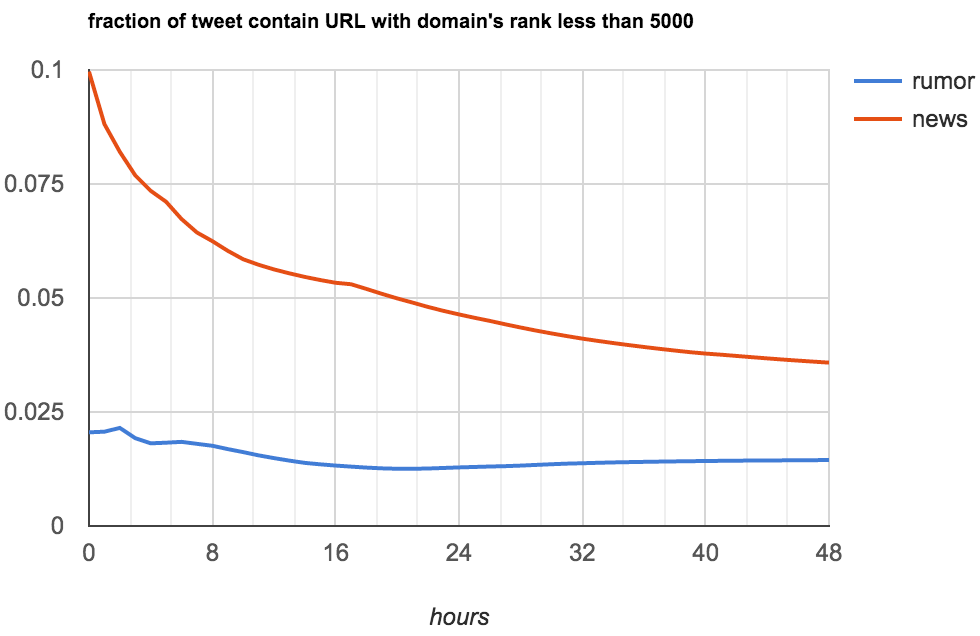
\includegraphics[width=0.52\columnwidth]{images/url5000.png}
\caption{The Fraction of Tweets Containing URL with Top 5000 Domain}
\label{fig:Url5000}
\end{figure}
\begin{figure}[!h]
\centering
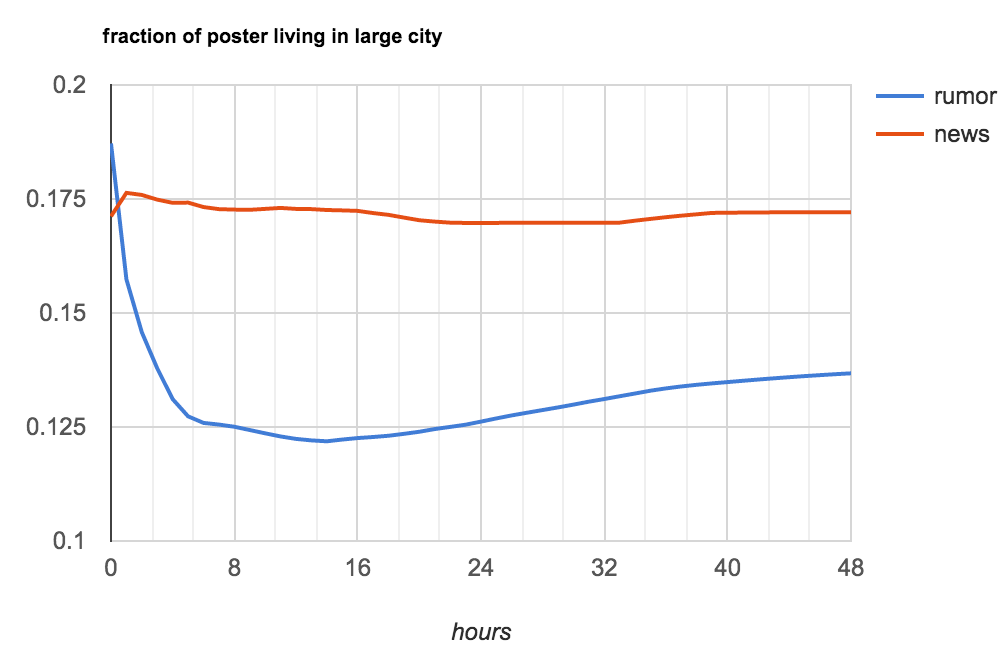
\includegraphics[width=0.52\columnwidth]{images/largecity.png}
\caption{The Fraction of Poster Living in Large City}
\label{fig:largecity}
\end{figure}
\newpage
  \section{ Dynamic Series-Time Structure (DSTS)} 
  In this section, we will introduce the Dynamic Series-Time Structure which is invented by Ma et al.~\cite{ma2015detect}. We use this structure to capture the temporal features.  
   \subsection{Time Stamps Generation} 
For an event $E_i$ we define $timeFirst_i$ as the start time of the event, $timeLast_i$ as the time of the last tweet of the event. We split each tweet $tw_{ij}$ into N time intervals according to thier creation time. The length of each time interval we define as follows: 

\begin{equation}
Interval(E_i)=\frac{\left \lceil { (timeLast_i-timeFirst_i) }\right \rceil}{N}
\end{equation}
And We define the index of time interval $TS(t_{ij})$ where a tweet $tw_{ij}$ which is created in time $t_{ij}$ should fall into, we define as follows:

\begin{equation}
TS(t_{ij})=\frac{\left \lfloor { (t_{ij}-timeFirst_i) }\right \rfloor}{Interval(E_i)}
\end{equation}

In our work $Interval(E_i)$ as we defined in Section \ref{sec:Time_Period_of_an_Event} as one hour and N is constant 48 hours for each event. 

   \subsection{Dynamic Series-Time Structure (DSTS)} 
Since we have all the time intervals of an event $E_i$ and we can generate a vector V($E_i$ ) of features for each time interval. And in order to capture the changes of feature over time, we should not only model the features in individual time intervals, but also model their differences between two time intervals. So the model of DSTS is represented as: 

\begin{equation}
 V(E_i)=(\textbf{F}^D_{i,0}, \textbf{F}^D_{i,1},..., \textbf{F}^D_{i,N},\textbf{S}^D_{i,1},..., \textbf{S}^D_{i,N})
\end{equation}
where the $\textbf{F}^D_{i,t}$ is the feature vector in time interval t of event $E_i$. $\textbf{S}^D_{i,t}$ is the difference between $\textbf{F}^D_{i,t}$ and $\textbf{F}^D_{i,t+1}$. V($E_i$ ) is the time series feature vector of the event $E_i$.
\begin{equation}
\textbf{F}^D_{i,t}=(\widetilde{ f}_{i,t,1},\widetilde{ f}_{i,t,2},...,\widetilde{ f}_{i,t,D})
\end{equation}

\begin{equation}
\textbf{S}^D_{i,t}=\frac{\textbf{F}^D_{i,t+1}-\textbf{F}^D_{i,t}}{Interval(E_i)}
\end{equation}
We use Z-score which is implemented by sklearn to normalize feature values .
\begin{equation}
\widetilde{f}_{i,t,k}=\frac{f_{i,t+1,k}-\overline{f}_{i,k}}{\sigma(f_{i,k})}
\end{equation}
where $f_{i,t,k}$ is the k-th feature in time interval t of the event $E_i$ in time interval t. $\overline{f}_{i,k}$ is the mean of the feature k of the event $E_i$ and $\sigma(f_{i,k})$ is the standard deviation of the feature k over all time intervals. We skip this step if we use random forest or decision trees, because they do not need feature normalization.

  \section{ Features} 
 
 In this section, we will introduce the the features of time series model. We use a collection of features based on previous works 
\cite{castillo2011information}\cite{gupta2014tweetcred} \cite{yang2012automatic}\cite{liu2015real}\cite{madetecting}\cite{ma2015detect} \cite{mendoza2010twitter}\cite{wu2015false}\cite{jin2013epidemiological}. They are totally 50 features shown in Table \ref{tab:full_features}. These features are extracted not only from Twitter interface but also from other external websites like bluecoat.com which are mentioned in Section \ref{cha:Data_Collection}. 
\subsection{Text Features}
Text features set is a normal feature set of tweets' content. It contains 16 features as shown in Table \ref{tab:full_features}. The difference between the text features in single tweet model and in time series model is, in time series model, the features is the ratio of tweets containing some features or average number of some features. For example LengthOfTweet in single tweet model means the length of a tweet, but in time series model it means the average length of tweets in certain time internals.  

NumOfChar is the average number of individual characters of tweets. It is case sensitivity. The average number of characters of rumor is 34 and news is 36.
\subsection{Twitter Features}
Twitter features are the features of Twitter's unique functions like hashtag or mention.
And we add 3 new features about the URLs of the tweets. The first one is the WOT Score which is crawled from the APIs of website wot.com\footnote{https://www.mywot.com/en/api}. WOT is short for Web of Trust and it scores the domains' credibility and safety. The second one is catalog of domain which I crawled from the bluecoat.com\footnote{http://sitereview.bluecoat.com/}. I simply group them into 2 types: news sites or non-news sites. The last one is the rank of the domain which I crawle from alexa.com\footnote{http://www.alexa.com/siteinfo/bbc.com}. I also split them into 2 groups: rank less than 5000 or rank higher than 5000. In our experiment, those 3 features about URLs have better performance than other original Twitter functions like hashtag or mention.
\subsection{User Features}
User's features are also similar with other pervious works. We add one new feature which can only get from the website interface, is how many photos has been posted by the user \emph{(UserNumPhoto)}. And another user feature which has good performance is whether the user lives in a large city. We use the list of large city in the report of demographia\footnote{http://www.demographia.com/db-worldua.pdf}.  
\subsection{Epidemiological Modeling Features}
\label{sec:epide}
In this section, we will introduce epidemiological model features. The work of Jin et al., as far as we know, is the first research which uses epidemiological model to analyze rumors' development on Twitter \cite{jin2013epidemiological}. They describe the propagation pattern of the rumors and news events with two models: SIS (Susceptible, Infected, Susceptible) and SEIZ (susceptible, exposed, infected, skeptic). 

\textbf{SIS} is one of the most popular epidemiological models. To adapt to the scenario of Twitter, we define a user who posts a tweet of relevant event as \textbf{(I)} infected, a user who dose not we define as \textbf{(S)} susceptible. But unlike in the normal epidemiological scenario where  infected nodes can be cured and return to susceptible, in Twitter the user once posts a tweet of the certain events, he will be classified into the infected component forever and can not return to susceptible again. At time t, the total number of population is $\Delta N(t)= I(t) + S(t)$ where $I(t)$ is the size of infected population and $S(t)$ is the size of susceptible population. As shown in Figure \ref{fig:SIS}, SIS model works as follows:

\begin{figure}[!h]
\center
\def\layersep{2.5cm}
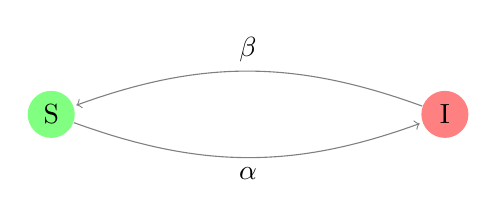
\begin{tikzpicture}[shorten >=1pt,->,draw=black!50, node distance=\layersep]
    \tikzstyle{every pin edge}=[<-,shorten <=1pt]
    \tikzstyle{neuron}=[circle,fill=black!25,minimum size=17pt,inner sep=0pt]
    \tikzstyle{input neuron}=[neuron, fill=green!50];
    \tikzstyle{output neuron}=[neuron, fill=red!50];
    % Draw the input layer nodes
     % This is the same as writing \foreach \name / \y in {1/1,2/2,3/3,4/4}
      \node[input neuron] (S) at (0,-1) {S};
     \node[ output neuron, xshift=5cm,yshift=-1cm] (I) {I};
      \path  (I) edge [above, bend right=20]node [sloped,midway,above] {$\beta$} (S) ;
     \path  (S) edge [below, bend right=20] node [sloped,midway,below]{$\alpha $}(I) ;
    % Annotate the layers
 \end{tikzpicture}
   \caption{SIS Model}
\label{fig:SIS}
\end{figure}
	
\begin{itemize}
\item A user who posts tweets about the certain event is regarded as infected.
\item A susceptible user has not tweeted about the certain event.
\item A susceptible user sees a tweet about the certain event from a infected users and he immediately retweets or posts a tweet about this event, and in that time he turns himself to infected.
\item Susceptible user will remain susceptible until he contacts (via tweet) with infected person.
\end{itemize}
we show SIS model mathematical as follow:
\begin{equation}
\frac{d[S]}{dt}=- \beta SI+\alpha I
\end{equation}
\begin{equation}
\frac{d[I]}{dt}= \beta SI-\alpha I
\end{equation}

SIS model assumes that a susceptible user once exposed to a infected user turns to infected immediately. That is one reason of this model why it dose not fit to Twitter. In fact when twitter users see tweets, they  their judgment to  truth of the information and they can decide whether further spreading the tweet or ignoring them.

Another popular model is SIR which contains one more term than the SIS. The definitions of \textbf{(S)} and \textbf{(I)} are the same in SIS, but the term \textbf{(R)} stands for recover. Once a susceptible user is recovered, he will be removed from the susceptible component and he can not be infected again. But we can not get a reasonable explanation of the term R if we model them as an event spreading on Twitter.

Because of the shortcomings of above two models, F. Jin et al. test SEIZ model which is referenced from Bettencourt et al.\cite{bettencourt2006power}. 
\begin{figure}[!h]
\center
\def\layersep{2.5cm}
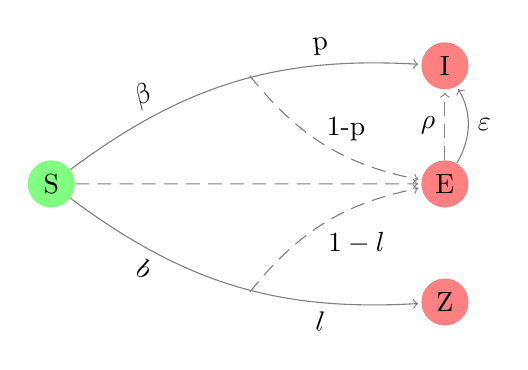
\begin{tikzpicture}[shorten >=1pt,->,draw=black!50, node distance=\layersep]
    \tikzstyle{every pin edge}=[<-,shorten <=1pt]
    \tikzstyle{neuron}=[circle,fill=black!25,minimum size=17pt,inner sep=0pt]
    \tikzstyle{input neuron}=[neuron, fill=green!50];
    \tikzstyle{output neuron}=[neuron, fill=red!50];
    \tikzstyle{miss node}=[inner sep=0,minimum size=1];
    % Draw the input layer nodes
     % This is the same as writing \foreach \name / \y in {1/1,2/2,3/3,4/4}
      \node[input neuron] (S) at (0,-2.5) {S};
      \node[ output neuron,  xshift=5cm,yshift=-1cm] (I) {I};
      \node[ output neuron,  xshift=5cm,yshift=-2.5cm] (E) {E};
      \node[ output neuron,  xshift=5cm,yshift=-4cm] (Z) {Z};
       \node[ miss node,  xshift=2.5cm,yshift=-1.1cm] (X) {};
       \node[ miss node,  xshift=2.5cm,yshift=-3.9cm] (X2) {};

	\path  (X) edge [dash pattern=on5pt off3pt,below, bend right=20] node [midway,right,xshift=-0.1cm,yshift=0.2cm]{1-p}(E) ;
 
      \path  (S) edge [above, bend left=20]node [sloped,near start,above] {$\beta$} node [sloped,near end,above] {p}  (I) ;
      \path  (E) edge [right, bend right=30] node [midway,right]{$\varepsilon $}(I) ;
      \path  (E) edge [dash pattern=on5pt off3pt] node [midway,left]{$\rho$}(I) ;
      \path  (S) edge [dash pattern=on5pt off3pt]  (E) ;
      \path  (S) edge [above, bend right=20]node [sloped,near start,below] {$b$} node [sloped,near end,below] {$l$}  (Z) ;
	\path  (X2) edge [dash pattern=on5pt off3pt,below, bend left=20] node [xshift=0.4cm]{$1-l $}(E) ;
	\end{tikzpicture}
   \caption{SEIZ Model}
\label{fig:SEIZ}
\end{figure}
 To adapt to Twitter context, the compartments of the SEIZ model can be mapped like this: \textbf{(S)}usceptible is a user who has not been exposed to the event, in the other word, he dose not see any tweets about the certain event yet. \textbf{(I)}nfected  means a user has posted tweets about the certain events, \textbf{(Z)} skeptic is a user who has been exposed to the certain event but he decides to ignore it and \textbf{(E)}xposed is a user who has been exposed to the certain event but he will post the tweets after delay.
 
 We show the model in Figure \ref{fig:SEIZ}. And the SEIZ works as follows:
 

 \begin{itemize}
\item People recruit from \textbf{(S)} susceptible compartment to skeptics with rate b. But with probability l, some of them directly deny the events and turn to \textbf{(Z)} skeptic compartments. Others with probability 1-l probability turn to \textbf{(E)} exposed compartment.
\item People recruit from \textbf{(S)} susceptible compartment to infected with rate $\beta$. But with probability p, some of them directly believe the events and repost it and turn them to be \textbf{(I)} infected compartments. Others  with probability 1-p probability turn to \textbf{(E)} exposed compartment.
\item  People from \textbf{(E)} exposed compartment may contact again with the Infected nods with $\rho$ probability and turn them to \textbf{(I)} infected compartment. And others have $\varepsilon$ probability turn into \textbf{(I)} infected compartment by themselves, for example driven by external shock.
\end{itemize}




We show SEIZ model mathematical as follows:
\begin{equation}
\frac{d[S]}{dt}=- \beta S\frac{I}{N}- b S\frac{Z}{N}
\end{equation}
\begin{equation}
\frac{d[E]}{dt}=(1-p)\beta S\frac{I}{N}+(1-l) b S\frac{I}{N}-\rho  S\frac{Z}{N}-\varepsilon E
\end{equation}
\begin{equation}
\frac{d[I]}{dt}=p\beta S\frac{I}{N}+\rho  S\frac{Z}{N}+\varepsilon E
\end{equation}
\begin{equation}
\frac{d[Z]}{dt}=lbS\frac{Z}{N} 
\end{equation}

\begin{table*}[!h]
 \centering
\scalebox{1}{
\begin{tabular}{@{\textbf{ }}lllllll@{}}
\toprule
\textbf{Symbol} & \textbf{Definition} \\ \midrule
$\beta$ & S-I contact rate\\  
b	&	 S-Z contact rate\\
$\rho $	&	E-I contact rate\\ 
$\varepsilon $   &	Incubation rate\\
$1/ \varepsilon $   &	Average Incubation Time\\
bl	&	Effective rate of S -> Z\\ 
$\beta \rho$   &	Effective rate of S -> I\\
b(1-l) & Effective rate of S -> E via contact with Z\\
$\beta (1-p)$	&	 Effective rate of S -> E via contact with I\\ 
l   &	 S->Z Probability given contact with skeptics\\
1-l &  S->E Probability given contact with skeptics\\
p	&	S->I Probability given contact with adopters\\
1-p	&	S->E Probability given contact with adopters \\ \bottomrule
\end{tabular}}
\caption{Parameters of SEIZ}
\label{tab:SEIZ_Para}
\end{table*}
The author presents an index of SEIZ called $R_{SI}$ as equation \ref{RSI}. It contains all rate values of SEIZ and related to the flux ratio of the \textbf{(E)} exposed compartment. If $R_{SI}$ is bigger than 1 means the influx of exposed compartment is bigger than the efflux. This index may be a good candidate of feature to analyze rumor spreading on Twitter.


\begin{equation}
\label{RSI}
R_{SI}=\frac{(1-p)\beta+(1-l)b}{\rho+\varepsilon}  
\end{equation}

We use Levenberg-Marquardt algorithm which we present in Section \ref{sec:LM} to learn the parameters of the SIS and SPEI. The fitting data is the tweets' volume of the 260 events  (130 rumors and 130 news). 
 In each time interval from $t_0$ to $t_n$, we fit the sequenced  tweets' volume from the beginning time $t_0$ to the current time interval $t_n$ of an event to SIS and SEIZ model and learn the parameters. From SIS we get two features $\beta_{n},\alpha_{n}$ and from SEIZ we get 7 features $\beta_{n},b_{n},l_{n},p_{n},\varepsilon_{n},\rho_{n},RSI_{n}$. We add them into our DSTS.
 
 
$FittingFunction_{SIS}(TweetVolume_{0},...,TweetVolume_{n})$->$\beta_{n},\alpha_{n}$%


$FittingFunction_{SEIZ}(TweetVolume_{0},...,TweetVolume_{n})$->$\beta_{n},b_{n},l_{n},p_{n},\varepsilon_{n},\rho_{n},RSI_{n}$


 We show 4 examples as following two rumors in Figures \ref{fig:SIS-rumor1} and \ref{fig:SIS-rumor2} and two news in Figures \ref{fig:SIS-news1} and \ref{fig:SIS-news2}. It is obvious that SEIZ is more appropriate than SIS to model in our application of Twitter, because the fitting error of SPEI is less than SIS. 


\begin{figure}[!h]

  \centering

\subfigure[SIS and SEIZ model for rumor 1]{\label{fig:SIS-rumor1}
\centering
  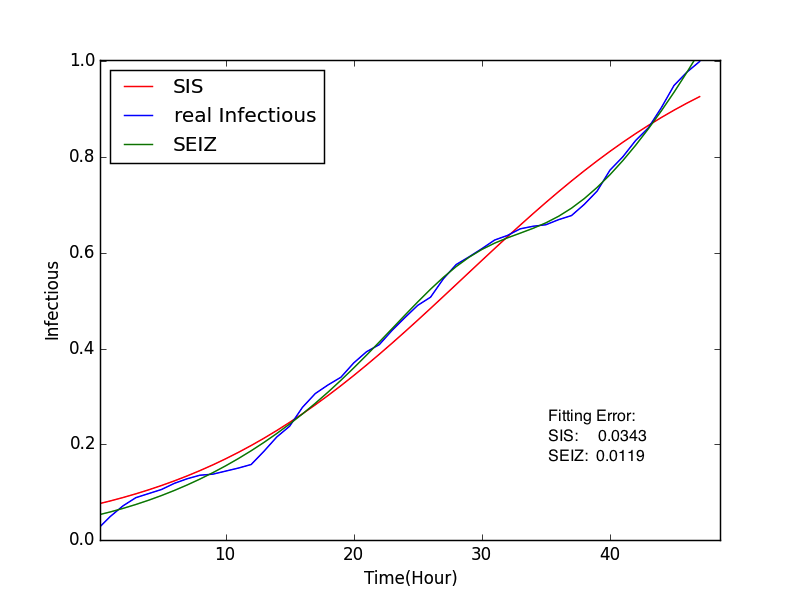
\includegraphics[width=0.45\columnwidth]{images/SISKKK.png}
} %
\subfigure[SIS and SEIZ model for rumor 2]{\label{fig:SIS-rumor2}
\centering
  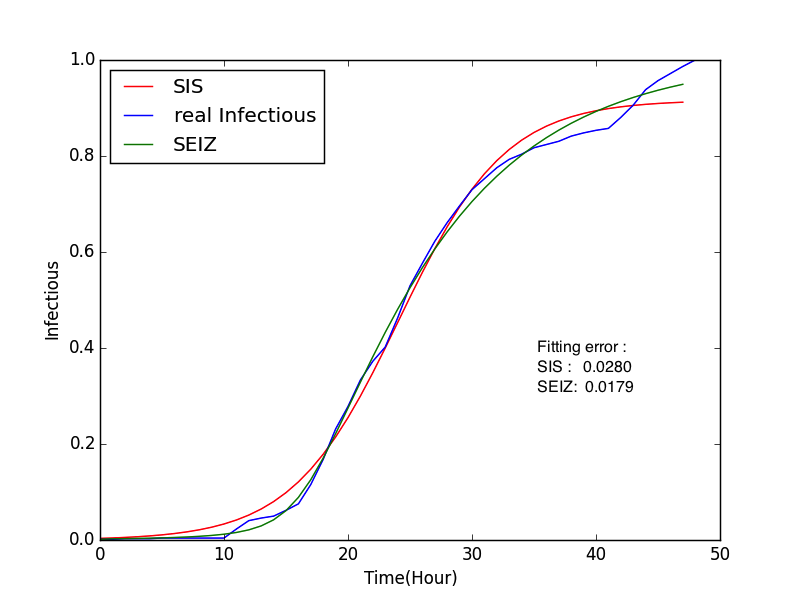
\includegraphics[width=0.45\columnwidth]{images/SIS449.png}
}
\subfigure[SIS and SEIZ model for news 1]{\label{fig:SIS-news1}
\centering
  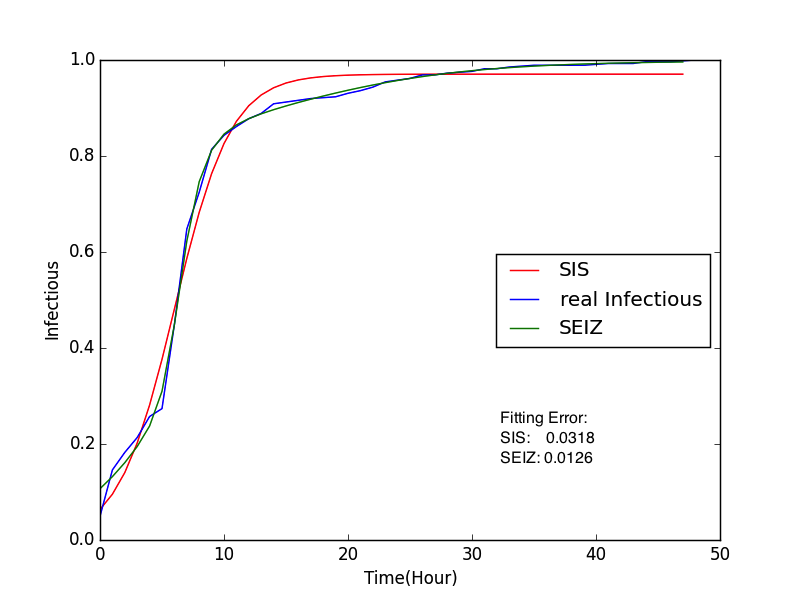
\includegraphics[width=0.45\columnwidth]{images/SISSHUMA.png}
}
\subfigure[SIS and SEIZ model for news 2]{\label{fig:SIS-news2}
\centering
  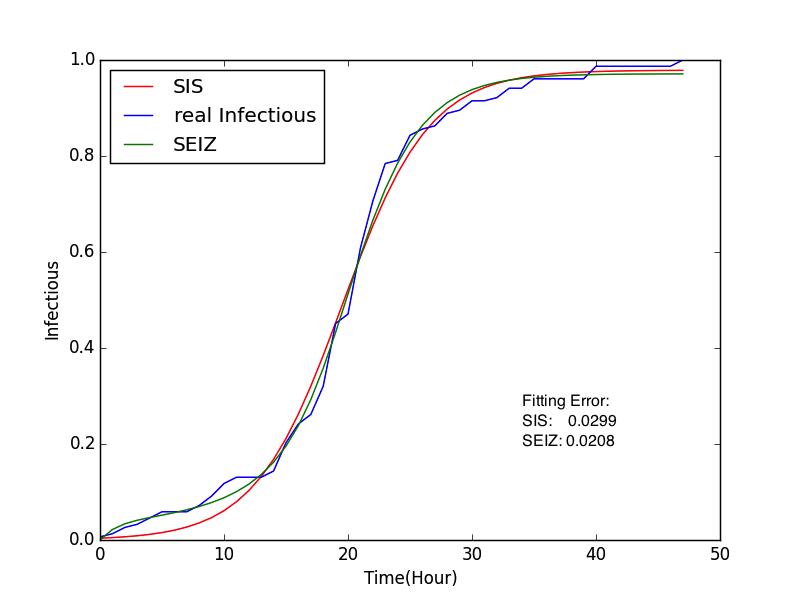
\includegraphics[width=0.45\columnwidth]{images/SIS1347.png}
}
\caption{Fitting results of SIS and SEIZ model of (a) Rumor: Robert Byrd was a member of KKK (b) Rumor: CNN altered a photograph of a shooter making him look white (c) News: Doctor announces Michael Schumacher is making process (d) News: Two U.S. sailors are arrested over an alleged rape of a Japanese woman on Okinawa}
\label{fig:SISModel}
\end{figure}

 
But if we fit the models of the first few hours with limited data, the result of learning parameters is not so accurate.  We show the performance of fitting these two model with only the first 10 hours tweets' volume in Figure \ref{fig:SISModelshort}. As we can see excepting the first one, the fitting results of other three are not good enough.

\begin{figure}[!h]

  \centering

\subfigure[SIS and SEIZ Model for Rumor \#1 with 10 Hours Data]{\label{fig:SIS-rumor1}
\centering
  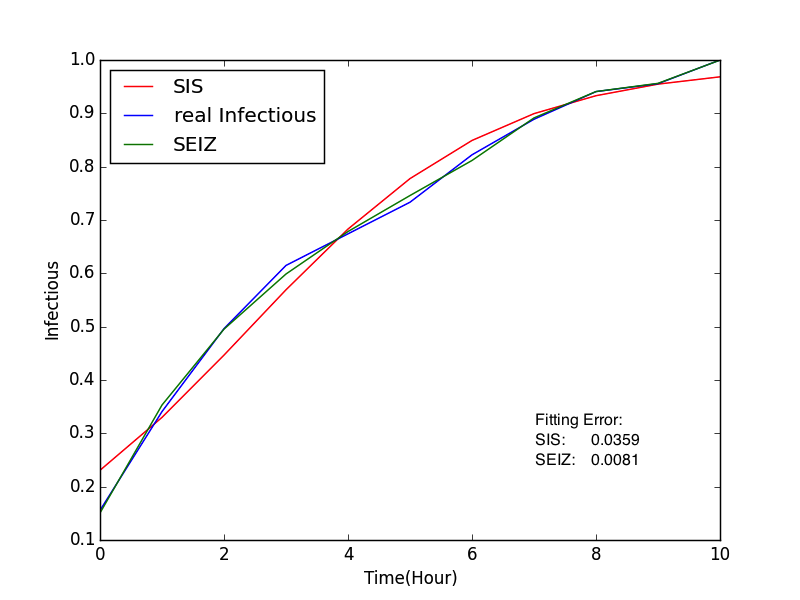
\includegraphics[width=0.45\columnwidth]{images/SISKKKshort.png}
} %
\subfigure[SIS and SEIZ Model for Rumor \#2 with 10 Hours Data]{\label{fig:SIS-rumor2}
\centering
  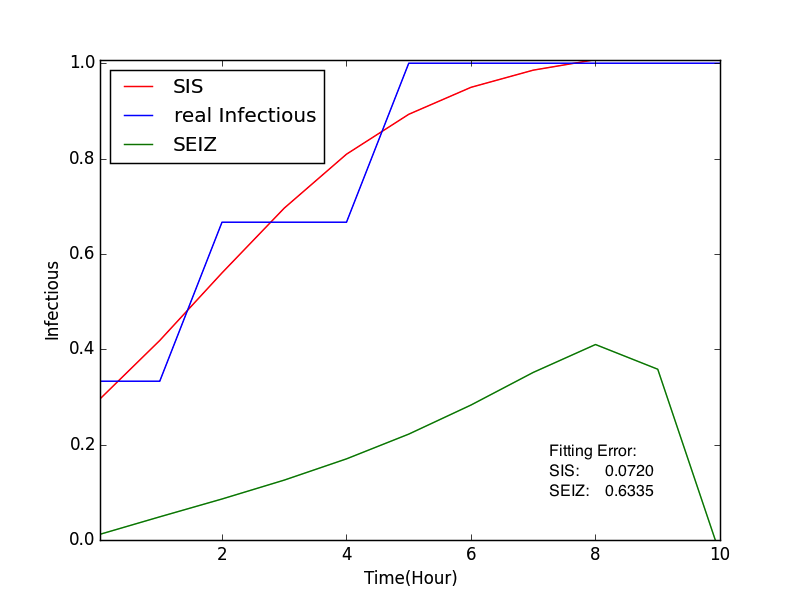
\includegraphics[width=0.45\columnwidth]{images/SIS449short.png}
}
\subfigure[SIS and SEIZ Model for News \#1 with 10 Hours Data]{\label{fig:SIS-news1}
\centering
  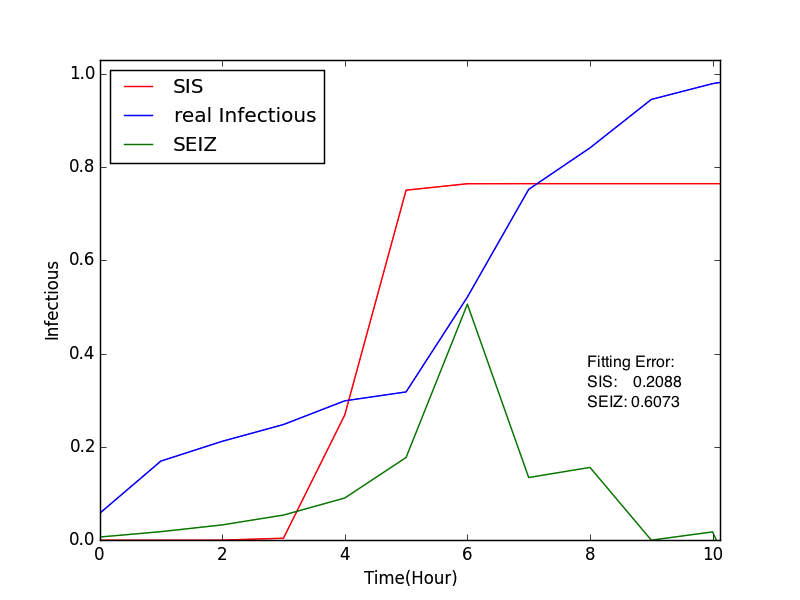
\includegraphics[width=0.45\columnwidth]{images/SISSHUMAshort.png}
}

\subfigure[SIS and SEIZ Model for News \#2 with 10 Hours Data]{\label{fig:SIS-news2}
\centering
  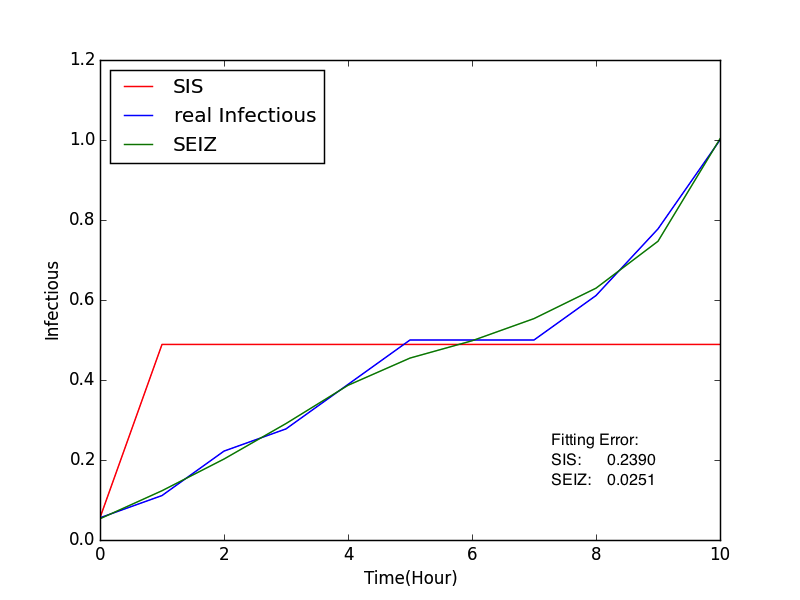
\includegraphics[width=0.45\columnwidth]{images/SIS1347short.png}
}
\caption{Fitting Results of SIS and SEIZ Model with Only First 10 Hours Tweets' Volume (same 4 stories as above)}
\label{fig:SISModelshort}
\end{figure}


\clearpage
\subsection{SpikeM model Features}
In this section, we will introduce the SpikeM feature set. Kwon et al. showed us another approach of representing the differences between the rumors' propagation pattern and the news events' propagation pattern on Twitter \cite{kwon2013prominent}. He adjusted the SpikeM Model and also used the parameters as features. 

SpikeM was first introduced by Yasuko Matsubara et al.\cite{conf/kdd/MatsubaraSPLF12} which can describe the pattern of information diffusion. We present it as follows:

\begin{equation}
\Delta B(n + 1) =p(n + 1)\cdot( U(n) \cdot  \sum ^n_{t=n_b}(\Delta B(t) + S(t))\cdot f(n+1-t) + \varepsilon )
\end{equation}
\begin{equation}
\label{periodic}
p(n) = 1-\frac{1}{2}P_a(\sin (\frac{2\pi}{P_p} (n+P_s)))+1)
\end{equation}

\begin{equation}
U(n + 1)=U(n)-\Delta {B(n + 1) }
\end{equation}
where
\begin{equation}
\label{decay}
f(\tau)=\beta \cdot \tau ^{-1.5}
\end{equation}
and initial conditions:
\begin{equation}
 \Delta B(0)=0 ,U(0) = N
\end{equation}
In addition, adding an external shock $S(n)$, a spike generated
at beginning time $n_b$. Mathematically, it is defined as follows:
\begin{equation}
\label{outs}
S(n) =\begin{cases}0 &(n \neq n_b)\\S_b  & (n =n_b)\end{cases} 
\end{equation}
As the definition: 
\begin{equation}
B(n) + U(n) = N
\end{equation}
The term of $\sum ^n_{t=n_b}(\Delta B(t) + S(t))$ is the total number of informed users at time n, so $\Delta B(n + 1) =p(n + 1)\cdot( U(n) \cdot  \sum ^n_{t=n_b}(\Delta B(t) + S(t))\cdot f(n+1-t) + \varepsilon )$ means that at time n+1 an infected node n randomly select a node m of all nodes and if the node m is susceptible the probability of m turning to infected is $\beta$, so it is a standard SI model. SpikeM extends the SI model from: 


 \begin{itemize}
\item a power-law decay term $f(\tau)=\beta \cdot \tau ^{-1.5}
$ in equation \ref{decay}. So the infection strength of the nodes which are earlier infected decreases in with a power-law decay pattern. 


\item a periodic interaction function in equation \ref{periodic}. It stands for that people have a periodic interaction patterns, for example people go to sleep at night, so they post much less tweets at night. Parameters $P_p$, $P_a$, and $P_s$ are the period, strength, and shift of the periodic interaction function.
\item $\varepsilon$ is the background noise term. 
\end{itemize}
\begin{table*}[!h]
 \centering
\scalebox{1}{
\begin{tabular}{@{\textbf{ }}lllllll@{}}
\toprule
\textbf{Symbol} & \textbf{Definition} \\ \midrule
N & total population of available bloggers\\ \midrule
$n_d$	&	duration of sequence\\
n	&	time-tick (n=0, . . . , $n_d$)\\\midrule
U(n)   &	count of \textbf{\underline{u}}n-informed bloggers\\
B(n)   &	count of informed \textbf{\underline{b}}loggers\\
$\Delta B(n)$	&	count of informed \textbf{\underline{b}}loggers at time n\\\midrule
f(n)   &	in\textbf{\underline{f}}ectiveness of a blog-post, at age n\\
$\beta$ & strength of infection\\
$\beta \cdot N$	&	"first-burst" size of infection\\\midrule
S(n)   &	volume of external \textbf{\underline{s}}hock at time n\\
$n_b$ & starting time of \textbf{\underline{b}}reaking news\\
$S_b$	&	strength of external shock at birth (time $n_b$)\\
$\varepsilon$	&	background noise \\\midrule
$P_a$ & strength of periodicity\\
$P_p$			& period of periodicity\\
$P_s$			& phase shift of periodicity\\ \bottomrule

\end{tabular}}
\caption{Parameters of SpikeM}
\label{tab:Features_Impsortance}
\end{table*}
But the SpikeM can't fit to the events with multi-pike like the Figure \ref{fig:KKK_part}. So the author think the term external shock $S(n)$ in equation \ref{outs} should not occur once but more. So they extend the SpikeM model by adding a periodic interaction function for the term external shock $S(n)$.

\begin{equation}
\Delta B(n + 1) =p(n + 1)\cdot( U(n) \cdot  \sum ^n_{t=n_b}(\Delta B(t) +  \bar{S}(t))\cdot f(n+1-t) + \varepsilon )
\end{equation}
\begin{equation}
\label{periodic}
p(n) = 1-\frac{1}{2}P_a(\sin (\frac{2\pi}{P_p} (n+P_s)))+1)
\end{equation}

\begin{equation}
U(n + 1)=U(n)-\Delta {B(n + 1) }
\end{equation}
\begin{equation}
\label{decay}
f(\tau)=\beta \cdot \tau ^{-1.5}
\end{equation}
The external shock $S(n)$ is added a periodic interaction function
\begin{equation}
\label{outs}
\bar{S}(t)=S(t)+q(t)
\end{equation}
\begin{equation}
q(t) =  q_a(\sin (\frac{2\pi}{q_p} (t+q_s)))+1)
\end{equation}


\begin{table*}[!h]
 \centering
\scalebox{1}{
\begin{tabular}{@{\textbf{ }}lllllll@{}}
\toprule
\textbf{Symbol} & \textbf{Definition} \\ \midrule
$q_a$ & strength of periodicity of the external shock\\
$q_p$			& period of periodicity of the external shock\\
$q_s$			& phase shift of periodicity of the external shock\\ \bottomrule

\end{tabular}}
\caption{New Parameters of Extended SpikeM}
\label{tab:Features_Impsortance2}
\end{table*}
Same approach as fitting SIS model, we learn the parameters of SpikeM model with Levenberg-Marquardt algorithm. We fit the sequenced tweets' volume from the beginning time the $t_0$ to the current time interval $t_n$ of an event to the model. The output parameters are used as the features adding into DSTS. We use $p_a$,  $p_p$, $p_s$ and $q_a$, $q_p$, $q_s$ as features. We show 4 examples of the SpikeM fitting result in Figure \ref{fig:SPikeModel}. But SpikeM has the same problem as fitting SIS or SEIZ model, if we test only within 10 hours data the results are much worse than the results with full 48 hours showing in Figure \ref{fig:SpikeMModelshort}.

\begin{figure}[!h]

  \centering

\subfigure[SIS and SEIZ Model for Rumors \#1]{\label{fig:SPikeM-rumor1}
\centering
  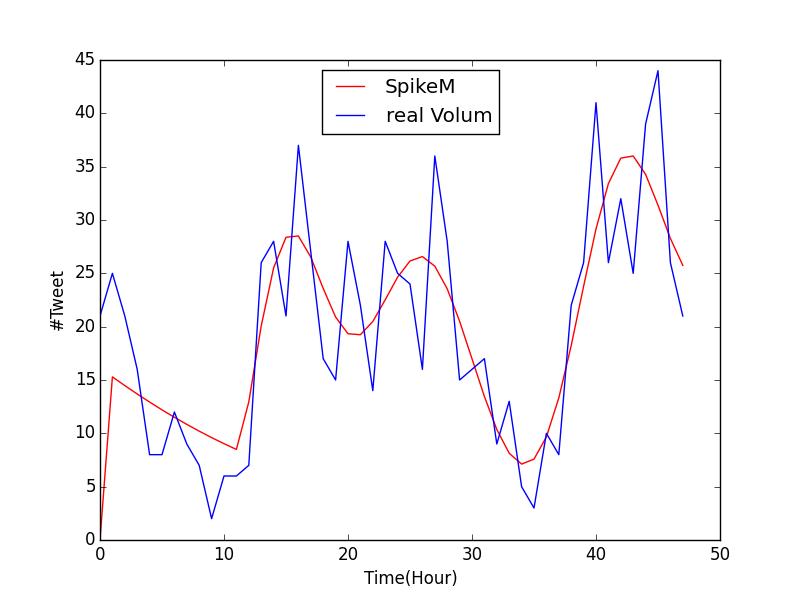
\includegraphics[width=0.48\columnwidth]{images/SpikeM_kkk.png}
} %
\subfigure[SIS and SEIZ Model for Rumors \#2 ]{\label{fig:SPikeM-rumor2}
\centering
  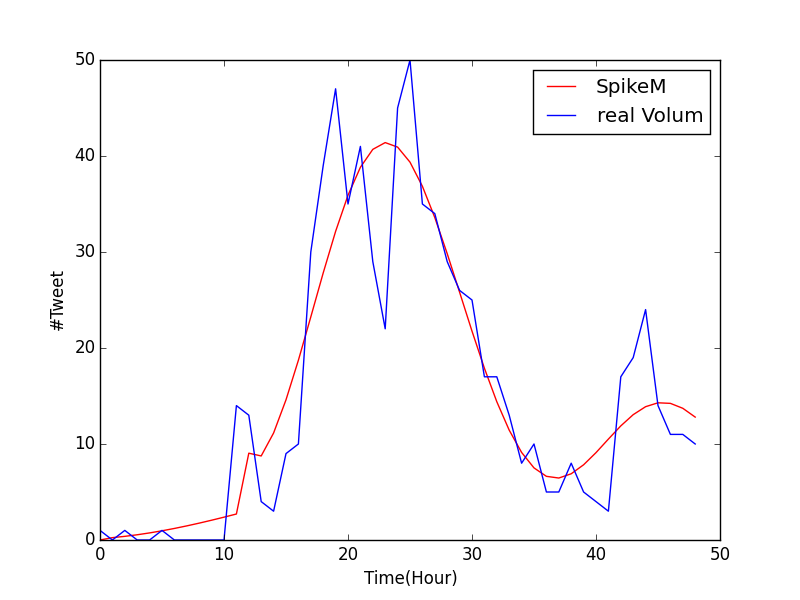
\includegraphics[width=0.48\columnwidth]{images/SpikeM_449.png}
}
\subfigure[SIS and SEIZ Model for News \#1]{\label{fig:SPikeM-news1}
   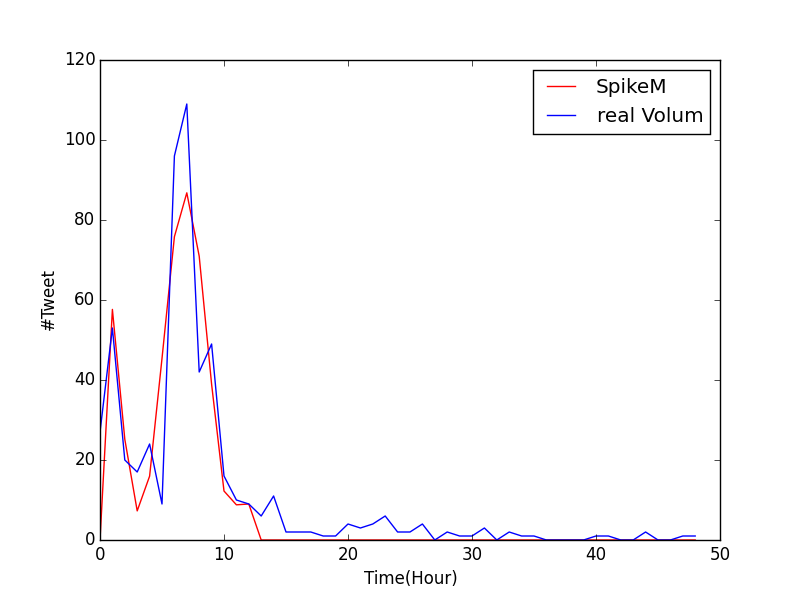
\includegraphics[width=0.48\columnwidth]{images/SpikeMSchuma.png}
}

\subfigure[SIS and SEIZ Model for News \#2 ]{\label{fig:SPikeM-news2}
   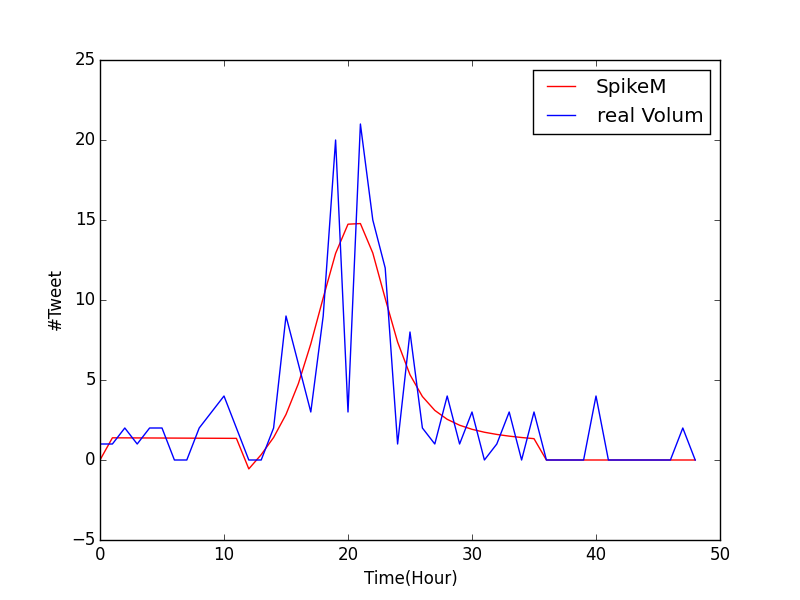
\includegraphics[width=0.48\columnwidth]{images/SpikeM_1347.png}
}
\caption{Fitting Results of SpikeM Model of (a) Rumor: Robert Byrd was a member of KKK (b) Rumor: CNN altered a photograph of a shooter making him look white (c) News: Doctor announces Michael Schumacher is making process (d) News: Two U.S. sailors are arrested over an alleged rape of a Japanese woman on Okinawa }
\label{fig:SPikeModel}
\end{figure}

\begin{figure}[!h]

  \centering

\subfigure[SIS and SEIZ Model for Rumor \#1 with 10 Hours Data]{\label{fig:SPikeM-rumor1}
\centering
  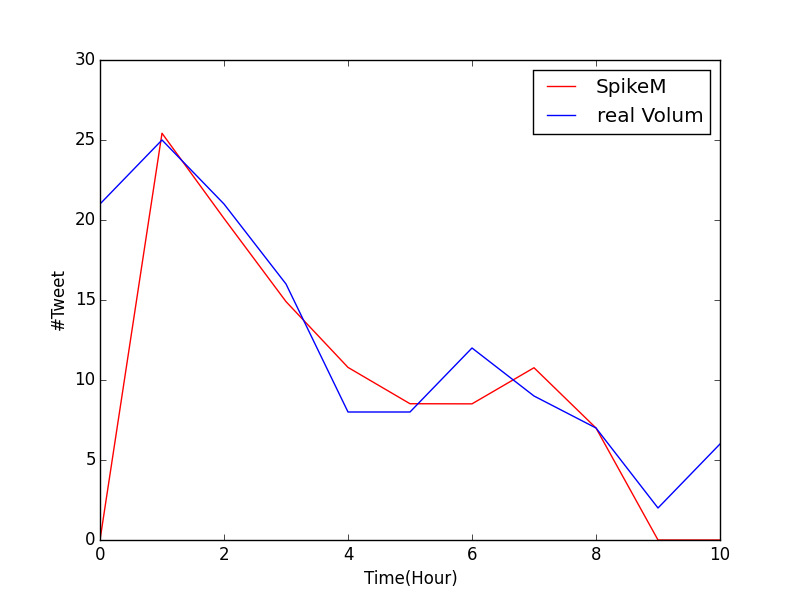
\includegraphics[width=0.48\columnwidth]{images/SpikeMKKKshort.png}
} %
\subfigure[SIS and SEIZ Model for Rumor \#2 with 10 Hours Data]{\label{fig:SPikeM-rumor2}
\centering
  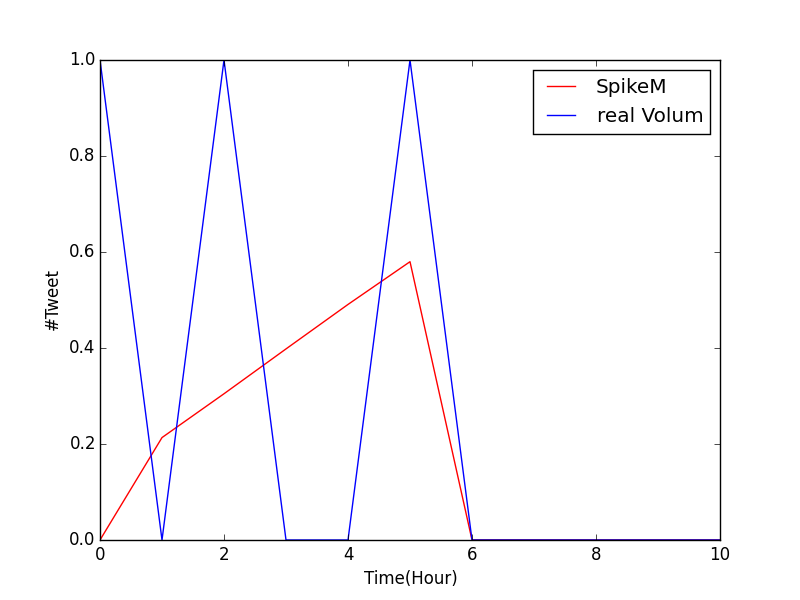
\includegraphics[width=0.48\columnwidth]{images/SpikeM492short.png}
}
\subfigure[SIS and SEIZ Model for News \#1 with 10 Hours Data]{\label{fig:SPikeM-news1}
\centering
  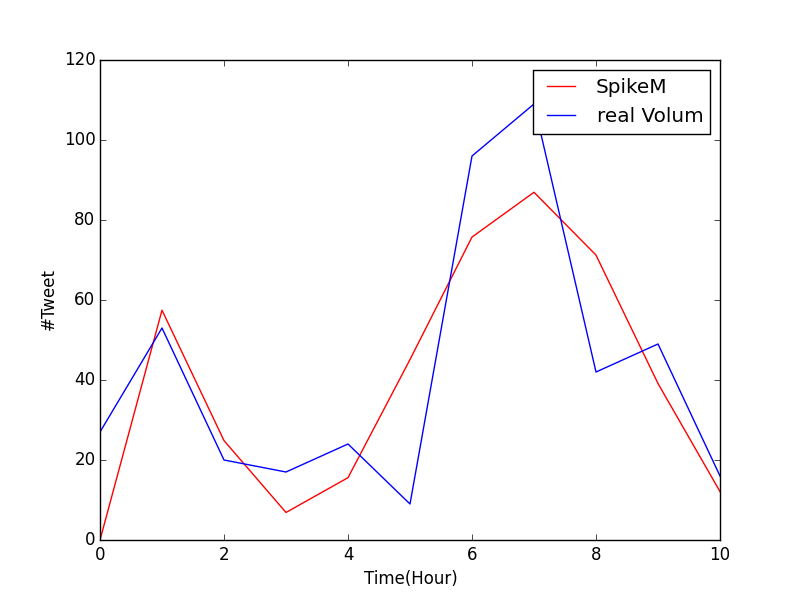
\includegraphics[width=0.48\columnwidth]{images/SpikeMSHUshort.png}
}

\subfigure[SIS and SEIZ Model for News \#2 with 10 Hours Data]{\label{fig:SPikeM-news2}
\centering
  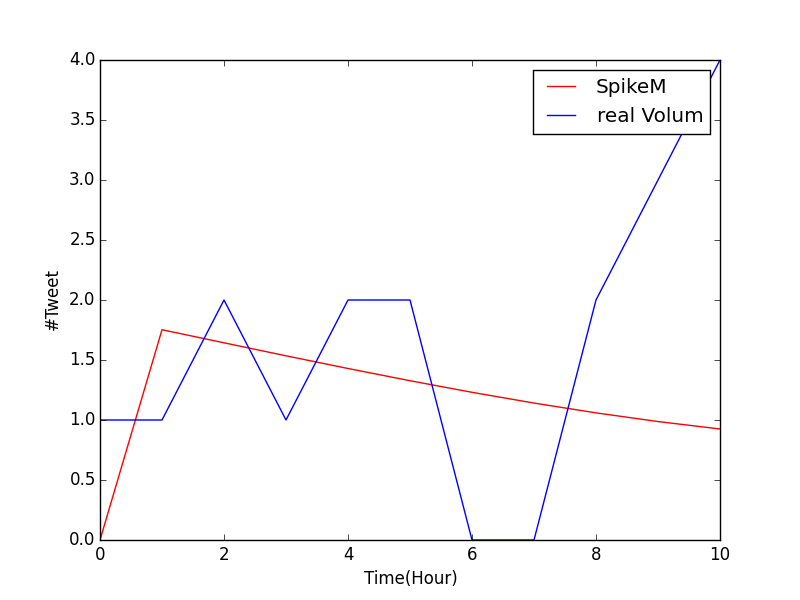
\includegraphics[width=0.48\columnwidth]{images/SpikeM1347short.png}
}
\caption{Fitting results of SpikeM Model with First 10 Hours data (same stories as above) }
\label{fig:SpikeMModelshort}
\end{figure}

\clearpage
\subsection{CrowdWisdom Features}
\emph{CrowdWisdom} feature comes from Liu et al. work \cite{liu2015real} but not same. The core idea is using the public's common sense to detect the rumors. If there are more people denying or doubting the truth of an event, this event is more likely to be a rumor. 
In the Liu et al. work, they use a extensive list of positive, negative and negation keywords and a set of rules like "negative words without negation words means the poster denies the event". And he uses the ratio between number of positive poster (supporter) over the negative poster (deny the events) as a feature.

We simplify from their work by only keeping a set of negative words. We call it "debunking words" like hoax, rumor, not true. Because we think the attitude of denying the event is already enough to distinguish rumors and news. In our test, "debunking words" is a good feature, but it needs 30 hours to "warm up". It is logical because crowds can debunk rumors but they need time to wait the professionals' advices or to unify the attitude the event.

\subsection{CreditScore Features}
To the best of our knowledge, \emph{CreditScore} feature is the first time to be used in rumor detection. Our pre-trained single tweet's creditability model predicts each tweet of the event. If the output is rumor related, we label it 1 otherwise 0. After that, we calculate the average \emph{CreditScore} of the events in certain time interval. We call this feature CreditScore. We will show it in Section \ref{creditscore} that \emph{CreditScore} is at least the second best feature in our experiment and it improves the performance of time series model especially in the first 24 hours.  
\subsection{Feature Selection} 
 \label{featusele}
 The RF feature selection is a filter method. Firstly we rank all features' average importance. Secondly we increase the number of features with the sequence of the rank, then we compare the performances which are shown in Figure \ref{fig:bestfeature}. The average accuracy of model is improved by adding more features, but after more than 9 features the accuracy stays stable instead of increasing. Therefore, we define the minimal feature set with good enough accuracy as BestSet with 9 features, we show them in Table \ref{bestfeature}.
 
  \begin{figure}[!h]
\centering
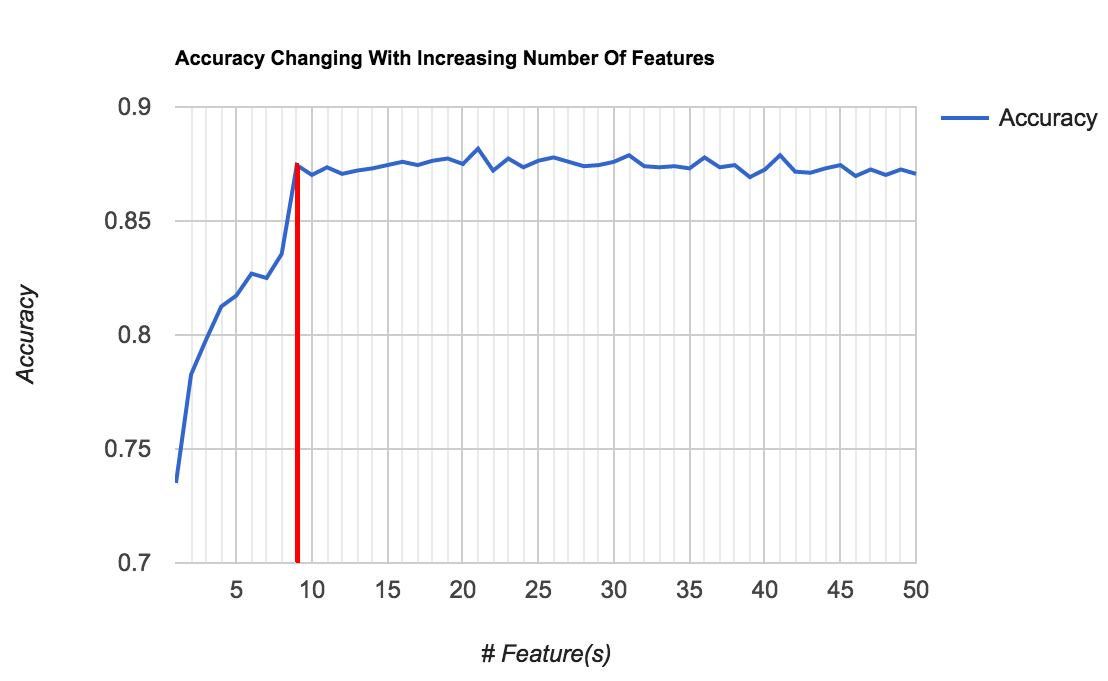
\includegraphics[width=\columnwidth]{images/featureseletion.png}
\caption{Accuracy Changing with Number Of Features }
\label{fig:bestfeature}
\end{figure}
 \begin{table}[!h]
\centering
\begin{tabular}{|l|}
\hline

 \textbf{Best Feature Set} \\\hline

 CreditScore \\ ContainNEWS \\

NumOfChar  \\ UserTweetsPerDays\\
QuestionExclamation  \\ UserReputationScore\\ 
 
WotScore  \\ Question\\
UserJoin\_date  \\ \bottomrule 
 \end{tabular}
\caption{Best Features}
\label{bestfeature}
\end{table}
  
\clearpage
\begin{table*}[!h]
\small
\centering
\scalebox{0.8}{
 \begin{tabular}{@{}lllllll@{}}
 \toprule
 \textbf{Category} & \textbf{Feature} & \textbf{Description}\\ \midrule
 Twitter Features& Hashtag & \% of the tweets containing \#hashtag  \cite{castillo2011information}\cite{liu2015real}\cite{qazvinian2011rumor}\cite{gupta2014tweetcred}\cite{liu2015real}\\
 		& Mention &  \% of the tweets mentioning others @user  \cite{castillo2011information}\cite{liu2015real}\cite{qazvinian2011rumor}\cite{gupta2014tweetcred}\cite{liu2015real}\\
 		& NumUrls &  \# of url in the tweet  \cite{castillo2011information}\cite{qazvinian2011rumor}\cite{gupta2014tweetcred}\cite{yang2012automatic}\cite{liu2015real}\\
 		& Retweets & average times of tweets have been retweeted \cite{liu2015real} \\ 
 		& IsRetweet & \% of tweets are retweeted from others \cite{castillo2011information}\cite{gupta2014tweetcred}\\
 		& ContainNEWS & \% of tweets containing URL and its domain's catalogue is News \cite{liu2015real}\\
 		& WotScore & average WOT score of domain in URL \cite{gupta2014tweetcred}\\
 		& URLRank5000 & \% of tweets contains URL whose domain's rank less than 5000 \cite{castillo2011information}\\
 		& ContainNewsURL & \% of tweets contains URL whose domain is News Website\\
\midrule
 Text Features & LengthofTweet & average length of tweets \cite{castillo2011information}\cite{gupta2014tweetcred}\\
    & NumOfChar & average number of individual characters of tweets \cite{castillo2011information}\cite{gupta2014tweetcred}\\
   & Capital &  average fraction of characters in Uppercase of tweets \cite{castillo2011information} \\
   & Smile & \% of tweets containing :->, :-), ;->, ;-) \cite{castillo2011information}\cite{gupta2014tweetcred}\\
   & Sad & \% of tweets containing :-<, :-(, ;->, ;-( \cite{castillo2011information}\cite{gupta2014tweetcred}\\
   & NumPositiveWords & average number of positive words \cite{castillo2011information}\cite{gupta2014tweetcred}\cite{yang2012automatic}\cite{liu2015real}\\
   & NumNegativeWords & average number of negative words \cite{castillo2011information}\cite{gupta2014tweetcred}\cite{yang2012automatic}\cite{liu2015real}\\
   & PolarityScores & average polarity scores of the Tweets \cite{castillo2011information}\cite{yang2012automatic}\cite{liu2015real}\\
   & Via & \% of tweets containing via \cite{gupta2014tweetcred}\\
   & Stock & \% of tweets containing \$  \cite{castillo2011information}\cite{gupta2014tweetcred}\\
   & Question & \% of tweets containing ? \cite{castillo2011information}\cite{liu2015real}\\
   & Exclamation & \% of tweets containing ! \cite{castillo2011information}\cite{liu2015real}\\
   & QuestionExclamation & \% of tweets containing multi Question or Exclamation mark \cite{castillo2011information}\cite{liu2015real}\\ 
   & I & \% of tweets containing first pronoun like I, my, mine, we, our    \cite{castillo2011information}\cite{gupta2014tweetcred}\cite{liu2015real}\\
   & You & \% of tweets containing second pronoun like U, you, your, yours  \cite{castillo2011information}\\ 
   & HeShe & \% of tweets containing third pronoun like he, she, they, his, etc.  \cite{castillo2011information}\\ \midrule
   User Features & UserNumFollowers  & average number of followers \cite{castillo2011information}\cite{gupta2014tweetcred}\cite{liu2015real}\\
 	& UserNumFriends  & average number of friends \cite{castillo2011information}\cite{gupta2014tweetcred}\cite{liu2015real}\\
 	& UserNumTweets  & average number of users posted tweets \cite{castillo2011information}\cite{gupta2014tweetcred}\cite{yang2012automatic}\cite{liu2015real}
\\
 	& UserNumPhotos  & average number of users posted photos \cite{yang2012automatic}\\
 	& UserIsInLargeCity  & \% of users living in large city \cite{yang2012automatic}\cite{liu2015real}\\
 	& UserJoinDate & average days since users joining Twitter \cite{castillo2011information}\cite{yang2012automatic}\cite{liu2015real}
\\
 	& UserDescription  & \% of user having description \cite{castillo2011information}\cite{yang2012automatic}\cite{liu2015real}
\\
 	& UserVerified  & \% of user being a verified user\cite{yang2012automatic}\cite{liu2015real}
\\
 	& UserReputationScore & average ratio of \#Friends over (\#Followers + \#Friends) \cite{liu2015real}\\   \midrule
 Epidemiological Features & $\beta_{SIS}$ & Parameter $\beta$ of Model SIS \cite{jin2013epidemiological}\\
 							& $\alpha_{SIS} $ & Parameter $\alpha$ of Model SIS \cite{jin2013epidemiological}\\
 							& $\beta_{SEIZ}$ & Parameter $\beta$ of Model SEIZ \cite{jin2013epidemiological}\\
 							& $b_{SEIZ}$ & Parameter b of Model SEIZ\cite{jin2013epidemiological}\\
 							& $l_{SEIZ}$ & Parameter l of Model SEIZ \cite{jin2013epidemiological}\\
 							& $p_{SEIZ}$ & Parameter p of Model SEIZ \cite{jin2013epidemiological}\\
 							& $\varepsilon_{SEIZ}$ & Parameter $\varepsilon$ of Model SEIZ \cite{jin2013epidemiological}\\
 							& $\rho_{SEIZ}$ & Parameter $\rho$ of Model SEIZ \cite{jin2013epidemiological}\\
 							& $R_{SI}$ & Parameter $R_{SI}$ of Model SEIZ \cite{jin2013epidemiological}\\
		\midrule	
 SpikeM Model Features & $P_s$ & Parameter $P_s$ of Model Spike \cite{kwon2013prominent}\\
 							& $P_a$ & Parameter $P_a$ of Model SpikeM \cite{kwon2013prominent}\\
 							& $P_p$ & Parameter $P_p$ of Model SpikeM \cite{kwon2013prominent}\\
 							& $Q_s$  & Parameter $Q_s$ of Model SpikeM \cite{kwon2013prominent}\\
 							& $Q_a$ & Parameter $Q_a$ of Model SpikeM \cite{kwon2013prominent}\\
 							& $Q_p$ & Parameter $Q_p$ of Model SpikeM \cite{kwon2013prominent}\\ \midrule	
 Crowd Wisdom Features & CrowdWisdom & \% of tweets containing "Debunking Words" \cite{liu2015real} \cite{zhao2015enquiring}\\ \midrule
 CreditScore Features & CreditScore & average CreditScore\\
 \bottomrule
 \end{tabular}}
 \caption{Features of Time Series Rumor Detection Model}
 \label{tab:full_features}
\end{table*}
\clearpage
  \section{Experimental Evaluation}
  \subsection{Datasets} 
  We use the same dataset as we mention in Section \ref{sec:dataset_single}, totally we collect 260 events and 130 of them are labeled as rumors. Their 
  categories are shown in Table \ref{tab:Tweet_con} and the time span of events are shown in Table \ref{tab:Tweet_Time}.

  \begin{table*}[!h]
 \centering
\scalebox{0.8}{
 \begin{tabular}{@{}cccccc@{}}
 \toprule
 \textbf{Event Categories} & \textbf{News} & \textbf{Rumor}&  \\ \midrule
 Politics & 43 & 49  \\ \midrule
 Science & 12  & 14 \\\midrule
 Art & 8 & 17  \\ \midrule
 Business & 13 & 19  \\ \midrule
 Health & 6 & 14  \\ \midrule
 Attacks & 27 & 7  \\ \midrule
 Disaster & 7 & 3  \\ \midrule
Other & 6 & 7  \\ \midrule \midrule
Total & 130 &130  \\
 	 \bottomrule
 \end{tabular}}
 \caption{Categories Of Rumors And News}
 \label{tab:Tweet_con}
\end{table*}
 
   We also extract 11,038 domains which are contained in the tweets in the 48 hours time period and we crawled these domains' categories in bluecoat.com\footnote{http://sitereview.bluecoat.com/sitereview.jsp\#/?search=bbc.com}, their ranks in alexa.com\footnote{http://www.alexa.com/siteinfo/bbc.com} and WOT score in wot.com\footnote{https://www.mywot.com/en/api}. The approach of defining the time period of events is the same as in Section \ref{sec:Time_Period_of_an_Event}.


\begin{table*}[!h]
 \centering
\scalebox{0.8}{
 \begin{tabular}{@{}cccccc@{}}
 \toprule
 \textbf{Type} & \textbf{Earliest Event} & \textbf{Latest Event}&  \textbf{Average Time Span (days)} \\ \midrule
 News & 21.02.2012 & 16.07.2016  &  4.5\\ \midrule
 Rumors & 20.10.2009  & 04.08.2016& 1679.6 \\
 	 \bottomrule
 \end{tabular}}
 \caption{Time Span of News and Rumors}
 \label{tab:Tweet_Time}
\end{table*}


\subsection{Experiment Setting } 
\label{cha:Data_Collection}


 \subsubsection{Classification Models } 
Same reason as in the single tweet's Creditability, we test the time series model also with 3 popular models: Decision Trees, SVM,  Random Forest and one more model: the multilayer perceptron (MLP). We show the optimized parameters in the Table \ref{tab:time_model_para}.  

\begin{table*}[!h]
 \centering
\scalebox{0.8}{
 \begin{tabular}{@{}l|l|l@{}}
 \toprule
 \multicolumn{1}{l|}{\textbf{Model}} &\multicolumn{1}{l|}{ \textbf{Parameters} }& \textbf{Value} \\ \midrule
 $TS-RF$ & Number of Trees & 350\\ \midrule
 $TS-SVM$ \cite{ma2015detect} & kernel  & radial basis function\\
 	& penalty parameter of the error term  & 3.0\\
 	& gamma  & $\frac{1}{50}$\\ \midrule
 Decision Trees & criterion & gini \\ \midrule
  MLP & alpha  & 0.0001\\
 	& activation function  & ReLU\\
 	& hidden layer sizes  & 2 layer(50 nodes each layer)\\
 	&weight optimization & adam\\ 
 \bottomrule
 \end{tabular}}
 \caption{Parameters of Classification models}
 \label{tab:time_model_para}
\end{table*}


 
  \subsection{Experiment Result} 
 In this subsection, we will present the experiment results. We test all models by using 10-fold cross validation with same shuffled sequence, the experiment result is shown in the Table \ref{tab:time_result}. Time Series Random Forest (TS-RF) is Random Forest with 9 selected time series features in Section \ref{featusele}, $TS-MLP_{all}$ is time series data structure with MLP, $TS-SVM$ is the baseline from Ma et al. work \cite{ma2015detect}, $TS-SVM_{all}$ is $TS-SVM$ with all features which I mentioned above, $TS-SVM_{Credit}$ is $TS-SVM$ with CreditScore, $TS-SVM_{SpikeM}$ is $TS-SVM$ with epidemiological features.
  
  As shown in the Table \ref{tab:time_result}, our model TS-RF has best performance in all case over time and CreditScore can significantly improve the performance of time series model in the first 24 hours of event. For example in the first hour, it improve the accuracy of the model from 0.65 of $TS-SVM$ to 0.71 of $TS-SVM_{Credit}$. And it is at least the second best feature in all case over time.
 
%\begin{table}[]
%\centering
%\begin{tabular}{|c|ccccccccc|}
%\hline
%\multicolumn{1}{|c|}{\multirow{2}{*}{Model}} & \multicolumn{9}{c|}{Accuracy in hours}                     \\ \cline{2-10} 
%\multicolumn{1}{|l|}{}& 1 & 6 &12& 18 & 24 & 30 & 36  & 42 & \multicolumn{1}{c|}{48} \\\hline
% $TS-RF$  & \textbf{0.8} &  \textbf{0.86} &  \textbf{0.86} &\textbf{0.87} & \textbf{0.87}& \textbf{0.87} &\textbf{0.88}&\textbf{0.88}&\textbf{0.91 }\\
%$TS-MLP_{all}$ &0.67& 0.74  & 0.74 & 0.78  &   0.77   &  0.81&0.79 &0.80&0.82 \\
%$TS-SVM$ \cite{ma2015detect}&0.65  &0.69 & 0.75& 0.77 &  0.77   &0.78 &0.80 &0.81 & 0.81  \\
%%$TS-SVM_{Credit}$&0.712 & 0.742  & 0.769  &0.792 &  0.800 & 0.788  &0.785 &0.777 &0.781\\
%%$TS-SVM_{SpikeM}$&0.685 & 0.704 & 0.754  & 0.75 &  0.758 &0.746  &0.765 &0.769  & 0.758\\
%$SVM_{static}$ &0.71& 0.79  & 0.81&0.78   &  0.75 &0.76& 0.79&0.75&0.76 \\   
%
%%$TS-SVM_{all}$ &0.738 & 0.777  & 0.796 & 0.777 &   0.765 &   0.762&   0.762&   0.750  & 0.746  \\
%
% \bottomrule           
%\end{tabular}
% \caption{Accuracy Of Different Models Over Time}
% \label{tab:time_result}
%\end{table}
%
%
%\begin{table}[]
%\centering
%\begin{tabular}{|c|ccccccccc|}
%\hline
%\multicolumn{1}{|c|}{\multirow{2}{*}{Model}} & \multicolumn{9}{c|}{Accuracy in hours}                     \\ \cline{2-10} 
%\multicolumn{1}{|l|}{}& 1 & 6 &12& 18 & 24 & 30 & 36  & 42 & \multicolumn{1}{c|}{48} \\\hline
%$TS-SVM$ \cite{ma2015detect}&0.65  &0.69 & 0.75& 0.77 &  0.77   &0.78 &\textbf{0.80} &\textbf{0.81} & \textbf{0.81}  \\
%$TS-SVM_{Credit}$&0.71 & 0.74  & 0.77  &\textbf{0.79} &  \textbf{0.80} & \textbf{0.79}  &0.79 &0.78 &0.78\\
%$TS-SVM_{SpikeM}$&0.69 & 0.70 & 0.76  & 0.75 &  0.76 &0.75 &0.77 &0.77  & 0.76\\
%
%$TS-SVM_{all}$ &\textbf{0.74} & \textbf{0.78}  & \textbf{0.80} & 0.78 &   0.77 &   0.76&   0.76&   0.75  & 0.75  \\ %\cline{1-10}
%%$SVM_{static}$ &0.707& 0.788  & 0.811&0.777   &  0.746 &0.761& 0.788&0.753&0.757 \\   
%
% \bottomrule           
%\end{tabular}
% \caption{Performance Of $TS-SVM$ with Different Sets of Features}
% \label{tab:Credit_time_result}
%\end{table}

\begin{table}[]
\centering
\begin{tabular}{|c|ccccccccc|}
\hline
\multicolumn{1}{|c|}{\multirow{2}{*}{Model}} & \multicolumn{9}{c|}{Accuracy in hours}                     \\ \cline{2-10} 
\multicolumn{1}{|l|}{}& 1 & 6 &12& 18 & 24 & 30 & 36  & 42 & \multicolumn{1}{c|}{48} \\\hline
 $TS-RF$  & \textbf{0.8} &  \textbf{0.86} &  \textbf{0.86} &\textbf{0.87} & \textbf{0.87}& \textbf{0.87} &\textbf{0.88}&\textbf{0.88}&\textbf{0.91 }\\
$TS-MLP_{all}$ &0.67& 0.74  & 0.74 & 0.78  &   0.77   &   \textit{\textbf{0.81}}&0.79 &0.80& \textit{\textbf{0.82}} \\

$TS-SVM$ \cite{ma2015detect}&0.65  &0.69 & 0.75& 0.77 &  0.77   &0.78 & \textit{\textbf{0.80}}& \textit{\textbf{0.81} }& 0.81  \\
$TS-SVM_{Credit}$& \textit{\textbf{0.71}} & 0.74  & 0.76  & \textit{\textbf{0.79} }&   \textit{\textbf{0.80}} & 0.79  &0.79 &0.78 &0.78\\

$TS-SVM_{Epi}$&0.67 & 0.73 & 0.73  & 0.73 &  0.75 &0.75  &0.74 &0.76 & 0.77\\

$TS-SVM_{SpikeM}$&0.69 & 0.70 & 0.75  & 0.75 &  0.76 &0.75 &0.77 &0.77  & 0.76\\
$TS-SVM_{all}$ &0.74 & \textit{ \textbf{0.78}}  &  \textit{\textbf{0.80}} & 0.78 &   0.77 &   0.76&   0.76&   0.75 & 0.75  \\

$SVM_{static}+Epi$ \cite{jin2013epidemiological} &0.60& 0.69  & 0.71&0.72   &  0.75 &0.78& 0.75&0.78&0.81 \\   

$SVM_{static}+SpikeM$ \cite{kwon2013prominent} &0.58& 0.68  & 0.72&0.73   &  0.77 &0.78& 0.78&0.79&0.77 \\   

$SVM_{static}$ \cite{yang2012automatic} &0.62& 0.70  & 0.70&0.72   &  0.75 &0.80& 0.79&0.78&0.77 \\   



 \bottomrule           
\end{tabular}
 \caption{Accuracy Of Different Models Over Time}
 \label{tab:time_result}
\end{table}
    \subsubsection{TS-RF VS Static Models} 

Firstly, we compare our time series model with the normal static feature model. We show the result in Table \ref{TVSF} the full 48 hours details in Appendix Table \ref{TSVSSFFULL} and in Figure \ref{fig:TVSF}. As we can see from the result that the accuracy of time series model overall is better than the static model. But after 32 hours the advantage of the time series is very limited. The reason may be after 32 hours the static model already has enough data to ignore the offset of features at the different time points. But the time series model still has benefits for detecting rumors at early stage of rumor spreading.  
 
\begin{table}[!h]
\centering
\begin{tabular}{|c|c c |c|}
\hline
Hour & TS-RF & Static RF & Difference \\ \hline
1    & 0.82              & 0.78         & 0.03       \\
6    & 0.86              & 0.8          & 0.06       \\
12   & 0.87              & 0.83         & 0.04       \\
18   & 0.88              & 0.83         & 0.05       \\
24   & 0.87              & 0.85         & 0.01       \\
30   & 0.88              & 0.85         & 0.03       \\
36   & 0.87              & 0.86         & 0.01          \\
42   & 0.88              & 0.88         & 0          \\
48   & 0.89              & 0.87         & 0.02      \\\hline

\end{tabular}
\caption{Accuracy: TS-RF VS Static RF}
\label{TVSF}
\end{table}

\begin{figure}[!h]
\centering
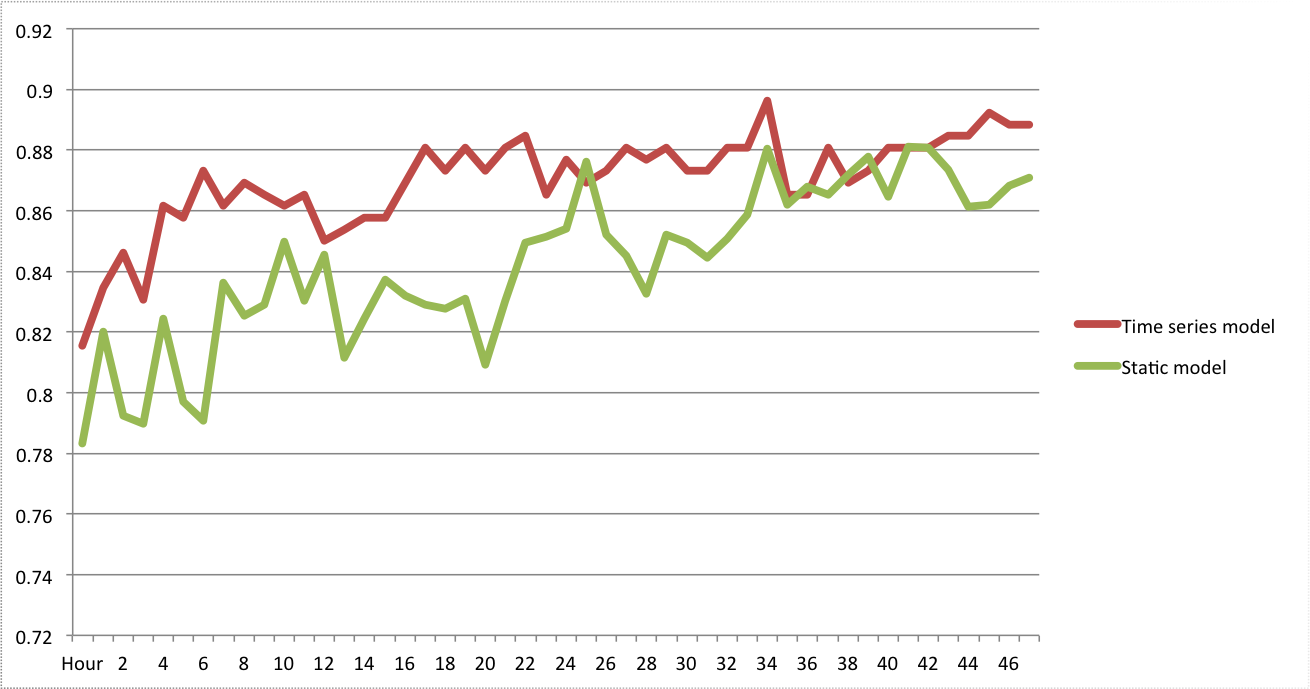
\includegraphics[width=0.8\columnwidth]{images/Vsstatic.png}
\caption{Accuracy: TS-RF VS Static RF}
\label{fig:TVSF}
\end{figure}

 
  \newpage
 \subsubsection{Feature Analyzing Over Time} 
 \label{featureanalyzing}
 In this subsection, we will present the performance of features changing over time. We rank the features' importance by using the method we introduced in Section \ref{random_forest}, the full result is shown in appendix Table \ref{tab:allfeaturerank}. First we split the features in 7 catalogues as in Table \ref{tab:full_features}: \emph{Tweet\_Feature}, \emph{User\_Feature}, \emph{Text\_Feature},  \emph{CreditScore}, \emph{SpikeM Features}, \emph{Epidemiological Features}, \emph{CrowdWisdom} and the \emph{BestSet}. The \emph{BestSet} is a combination of the top 9 most important features which is mentioned in Section \ref{featusele}. The results over 48 hours are in Figure \ref{fig:allfeature} .
 

 \begin{figure}[!h]
\centering
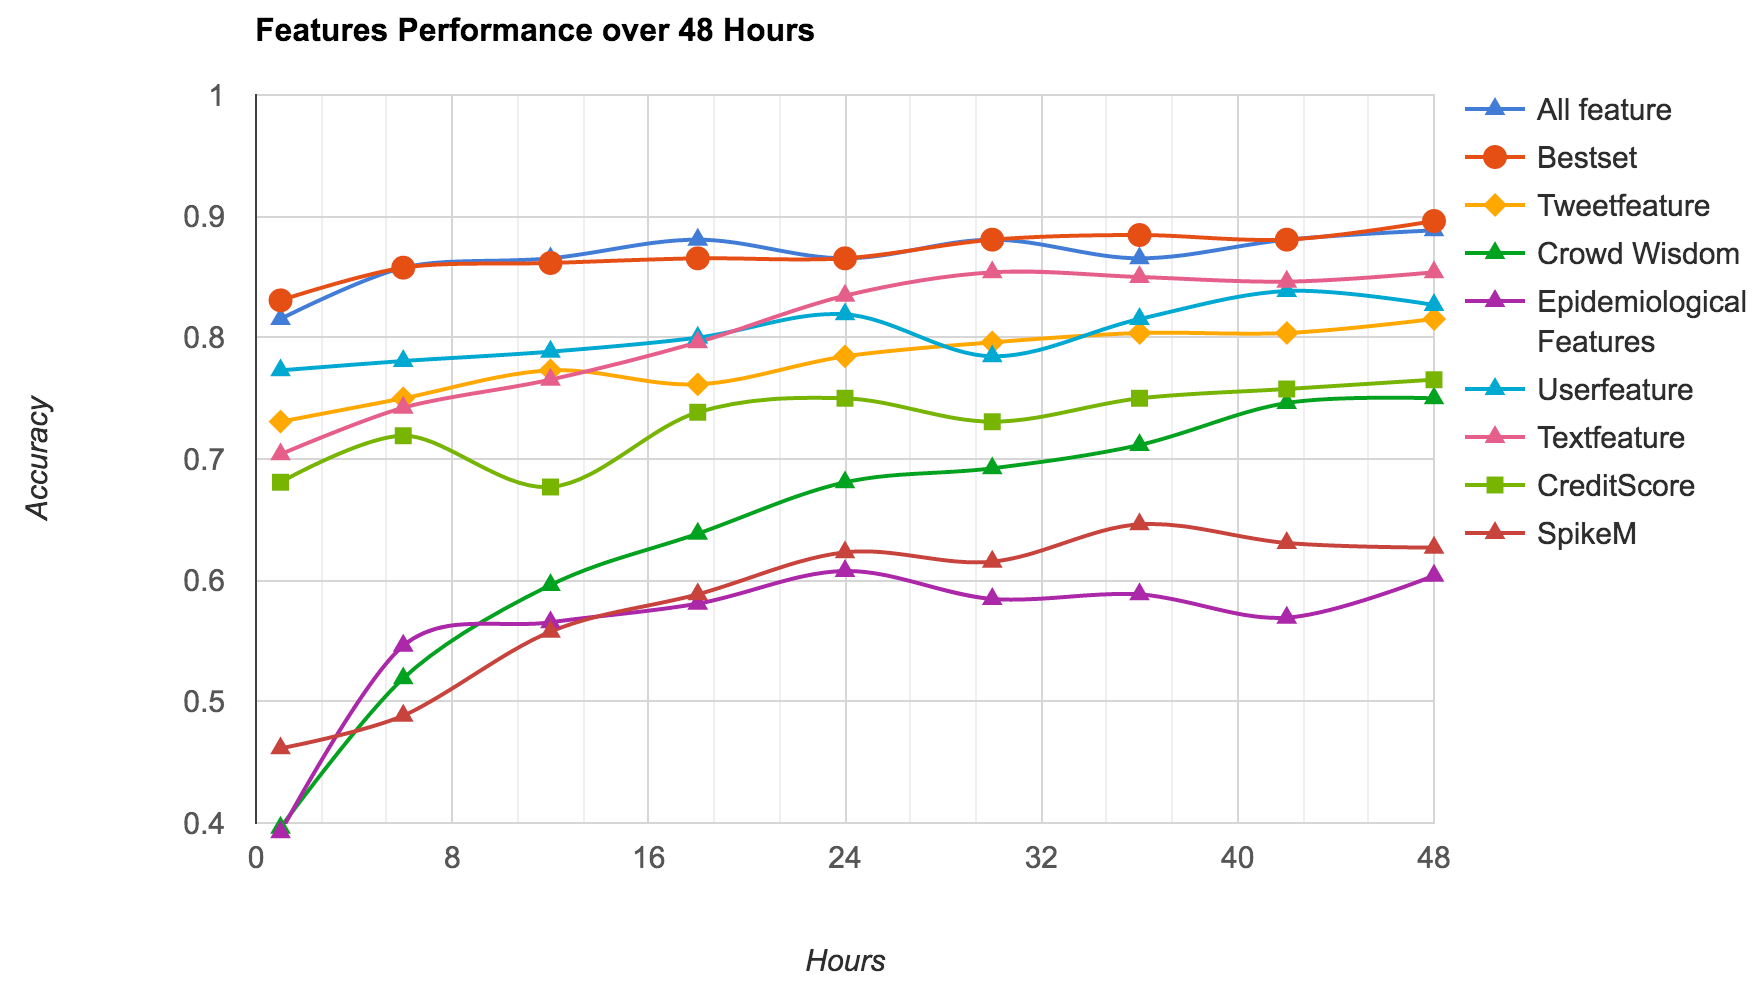
\includegraphics[width=\columnwidth]{images/allfeatures.png}
\caption{Accuracy of Different Groups of Features}
\label{fig:allfeature}
\end{figure}
 
 As we can see in Figure \ref{fig:allfeature} the best result on average over 48 hours in the \emph{BestSet} with top 9 features. Second one is the \emph{All features}. Except those two the best group feature is \emph{Text feature}. One reason is the text feature set has the largest group of feature with totally 16 features. But if look into each feature in text feature group we can see the best and the worst features are all in this set. \emph{User features set} and \emph{Twitter features set} are stable over time around 82\%. The performances of 3 different models (SIS, SEIZ and SpikeM) describing the propagation pattern of rumors and news are not ideal especially within 24 hours. \emph{CrowdWisdom} and \emph{CreditScore} both contain only one feature, but they already have impressive result comparing with the \emph{User feature} and \emph{Twitter feature}.
 \subsubsection{BestSet Features} 
\emph{BestSet} is a features set of 9 most important features which we mentioned in Section \ref{featusele}. On average \emph{BestSet} has the best performance.
 
 \subsubsection{Text Features} 
 \emph{Text features set} contains totally 16 features. The ranks of feature as shown in Table \ref{testfeaturerank}. The best one is \emph{NumOfChar} which is the average number of different characters in tweets. 
  
 \emph{PolarityScores} is the best feature when we tested the single tweets model, but its performance in time series model is not ideal. It is true that rumor contains more negative sentiment, but in an event (rumor or news) people can show their mixed views about this event \cite{mendoza2010twitter} \cite{starbird2014rumors} like discussing or denying, so the \emph{PolarityScores}'s performance becomes worse and worse over time. 
  \emph{Text feature} overall is the the best feature set.
 
 \begin{table}[!h]
 \centering
\scalebox{1}{
\begin{tabular}{@{\textbf{ }}ccccccccccccccccc@{}}
\toprule
\textbf{Features} & \multicolumn{10}{c}{\textbf{Ranks}} \\\hline
Hours & 1 & 6 & 12 & 18&24&30&36&42&48 & AVG\\\hline
 %ContainNEWS & 8 & 4 & 5& 4 & 4&2&2&2&2&3.48\\
NumOfChar			& 3& 3 & 4 & 3& 3& 8& 7&6 & 4& 4.29\\
QuestionExclamation		& 25& 16 & 2 & 1& 1& 1& 3& 7&5&4.79\\
%UrlRankIn5000			& 14& 13 & 7 & 11 & 7& 3& 1& 4&6&4.79\\
%WotScore			& 4 & 10& 6 & 10 & 10& 6& 9& 8&7&7.63\\ 
Question 			& 15 & 11& 13 & 7 & 5& 4& 8& 5&8&8.29\\ 
%Mention 			& 13 & 5& 10 & 14 & 13& 10& 12& 12&10&10.98\\
LengthOfTweet 			& 6 & 6& 9 & 6 & 14& 16& 13& 16&13&11.96\\ 
PolarityScores & 12 & 15& 23 & 28 & 33& 33& 34& 31&32&28\\

Stock 			& 34 & 44& 47 & 47 & 47& 47& 47& 47&48&46.15\\ 
Smile 			& 35 & 45& 45 & 48 & 48& 48& 48& 48&48&47.06\\ 
 
Sad 			& 36 & 46& 46 & 49 & 49& 49& 49& 49&49&47.9\\ 

\bottomrule
 \end{tabular}}
\caption{Rank of Part of Text Feature}
\label{testfeaturerank}
\end{table}
 \subsubsection{Twitter Features} 
   The performance of \emph{Twitter feature} is stable over time from the beginning to the end.

 The 3 best of \emph{Twitter Features} are all the features about the contained ULR in tweet: \emph{ContainNEWS}, \emph{UrlRankIn5000}, \emph{WotScore} showing in Table \ref{twitterfeaturerank}. It is quite reasonable that the news event would have higher probability to be reported by news websites or higher ranked website. And it is clear to see that their performances significantly improve after 24 hours.
 

 But the other original Twitter functions like the retweets or mention do not contribute much.
 

\begin{table}[!h]
\centering
\scalebox{1}{
\begin{tabular}{@{\textbf{ }}ccccccccccccccccc@{}}
\toprule
\textbf{Features} & \multicolumn{10}{c}{\textbf{Ranks}} \\\hline
Hours & 1 & 6 & 12 & 18&24&30&36&42&48 & AVG\\\hline
ContainNEWS & 8 & 4 & 5& 4 & 4&2&2&2&2&3.48\\
UrlRankIn5000			& 14& 13 & 7 & 11 & 7& 3& 1& 4&6&5.96\\
WotScore			& 4 & 10& 6 & 10 & 10& 6& 9& 8&7&7.63\\ 
%Question 			& 15 & 11& 13 & 7 & 5& 4& 8& 5&8&8.29\\ 
Mention 			& 13 & 5& 10 & 14 & 13& 10& 12& 12&10&10.98\\
Hashtag 			& 20 & 20& 15 & 18 & 16& 13& 15& 17&17&17.46\\ 
Retweets & 21 & 21& 27 & 38 & 42& 35& 31& 37&34&33.25\\
\bottomrule
 \end{tabular}}
\caption{Rank of Part of Twitter Feature}
\label{twitterfeaturerank}
\end{table}

\subsubsection{User Features} 
The performance of \emph{user features} is similar with the \emph{Twitter features}, they are both quite stable from the first hour to the last hour. But one difference is in the first few hours \emph{user feature} is the second best feature set after the \emph{AllFeatures set}.

As shown in Table \ref{userfeaturerank}, the best feature over 48 hours of user feature is \emph{UserTweetsPerDays} and it is the best feature overall in the first 4 hours, but its rank decreases with time going by. Others user features like UserReputationScore and UserJoinDate also has a better performance in the first fews hours. 

That means the sources (the poster in the first few hours) of news and rumors are quite different with each other. But with more and more users joining in the discussion, the bias of two groups of users becomes less. After 6 hours, we can better distinguish the rumors basing on the content of the tweet \emph{(text features)} than basing on the feature of the User.
 
\begin{table}[!h]
\centering
\scalebox{1}{
\begin{tabular}{@{\textbf{ }}ccccccccccccccccc@{}}
\toprule
\textbf{Features} & \multicolumn{10}{c}{\textbf{Ranks}} \\\hline
Hours & 1 & 6 & 12 & 18&24&30&36&42&48 & AVG\\\hline
UserTweetsPerDays & 0 & 1 & 1& 2 & 2&9&5&10&14&4.63\\
UserReputationScore	 & 1& 2 & 3 & 5 &6& 5& 6& 3&3&5.06\\
UserJoin\_date			& 5 & 8& 8 & 8 & 12& 14& 16& 11&9&10.58\\ 
UserVerified 			& 24 & 17& 12 & 16 & 17& 12& 11&14&19&16.25\\ 
 \bottomrule
 \end{tabular}}
\caption{Rank of Part of User Feature}
\label{userfeaturerank}
\end{table}
\subsubsection{SpikeM Features and Epidemiological Features}
The performances of these two feature sets are not so convincing. The feature $P_a$ from the SpikeM is the best one of them. 
The problem of these two models which we have already figured out in Section \ref{sec:epide} is that two models need enough data to fit the parameters. After 24 hours, model with epidemiological features with SpikeM can reach 60\% accuracy. In other words before 24 hour these is no clear propagation pattern of these events. In the work of Kwon et al. \cite{kwon2013prominent}, the durations of dataset which he uses are more than 60 days. In the work of Jin  et al. \cite{jin2013epidemiological}, they uses 160 hours' tweets' volume to fit the SEIZ models. Their data's durations are far larger than ours 48 hours.
 
 $P_a$ parameter from SpikeM is the only feature barely has some contributions for rumor detection in our experiment. It stands for the strength of periodicity in SpikeM.  Kwon  et al. add 3 more parameters $Q_a$,$Q_p$ and $Q_s$ to explain the periodicity of the external shock, but they do not produce same effect in our experiment, because 48 hours time period is too short to contain multi-pike pattern.

\begin{table}[!h]
\centering
\scalebox{1}{
\begin{tabular}{@{\textbf{ }}ccccccccccccccccc@{}}
\toprule
\textbf{Features} & \multicolumn{10}{c}{\textbf{Ranks}} \\\hline
Hours & 1 & 6 & 12 & 18&24&30&36&42&48 & AVG\\\hline
$P_a$ & 29 & 28 & 34& 30 & 33&24&23&21&23&25.75\\
$R_{SI}$	 & 47& 24 & 30 & 23 &36& 39& 38& 24&30&29.56\\
$\beta_{SIS}$			&49& 30 & 33& 28 & 31 & 36&28&33&25&30.15\\ 
$Q_a$  			& 44 & 47& 47 & 21 & 38& 40& 44&41&33&38.04\\ 
 \bottomrule
 \end{tabular}}
 \caption{Rank of Part of SpikeM Features and Epidemiological Features}
\label{SPikemfeaturerank}

 \end{table}
 
 \subsubsection{CreditScore}
 \label{creditscore}
 
\emph{CreditScore} is the output pre-trained Single Tweet Credibility Scoring model's in Section \ref{sec:single_nofeature}. As shown in Table \ref{tab:Rank_Credit}, excepting the first 4 hours \emph{CreditScore} is the best feature overall. In Figure \ref{fig:WCVSAF} we show the result of model without \emph{CreditScore} feature and model with full features set. Before the first 24 hours the model without \emph{CreditScore} has worse performance than the full feature set, so the \emph{CreditScore} feature contributes much for the early stage of rumor detecting. 

 \begin{figure}[!h]
\centering
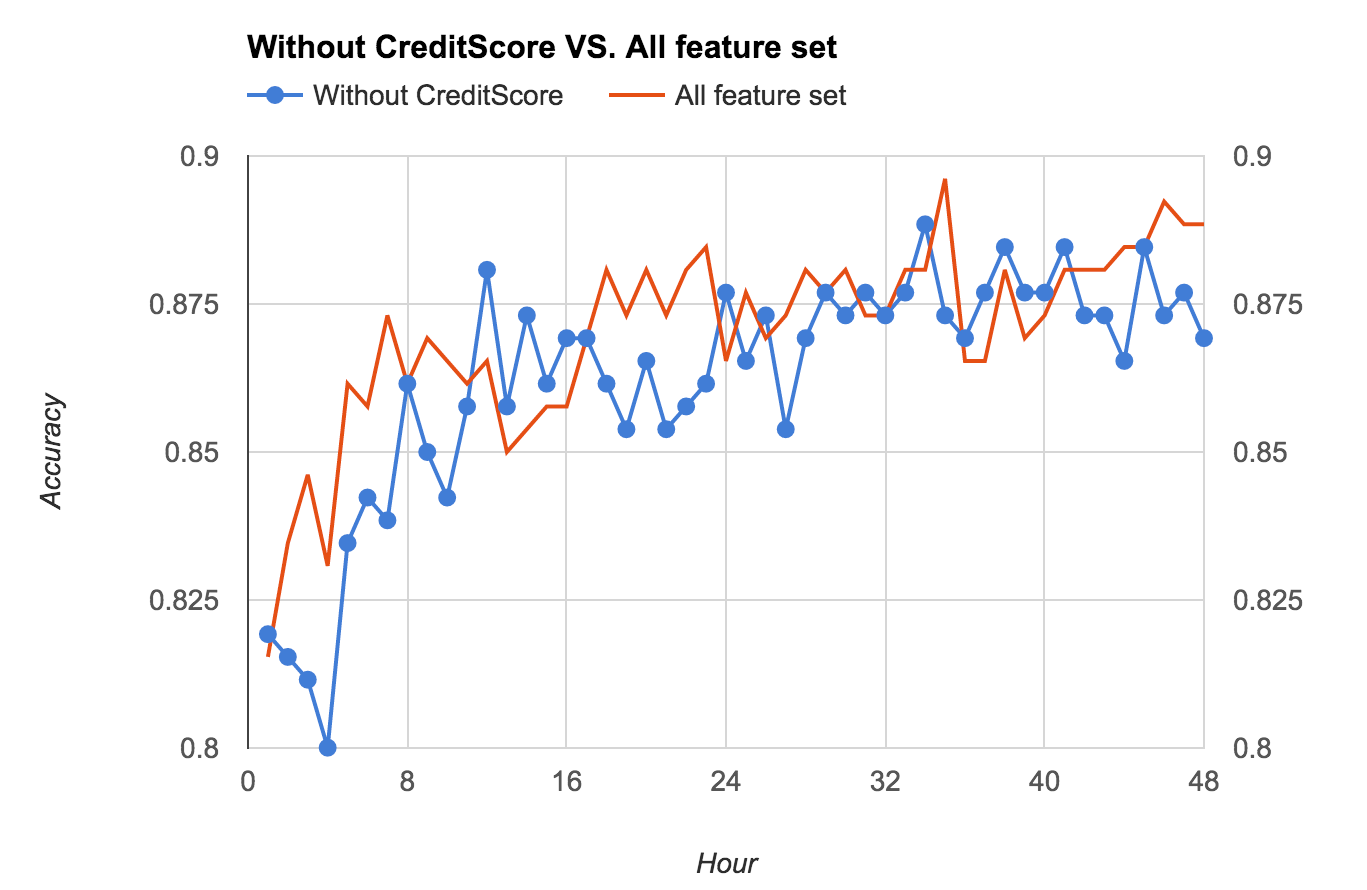
\includegraphics[width=\columnwidth]{images/WCVSAF.png}
\caption{Accuracy:Performance of Model with CreditScore VS Accuracy:Performance of Model without CreditScore}
\label{fig:WCVSAF}
\end{figure}

  \begin{table*}[!h]
 \centering
\scalebox{1}{
\begin{tabular}{@{\textbf{ }}cll@{}}
\toprule
\textbf{Hour} & \textbf{Rank} \\ \midrule
1 & 2\\
2			& 1\\
3			& 1\\
4			& 1\\
5			& 0\\ 
..  & 0\\ 
48 & 0\\ 
\bottomrule

\end{tabular}}
\caption{Ranks of CreditScore}
\label{tab:Rank_Credit}
\end{table*}
  
  \begin{table}[!h]
\centering
\scalebox{1}{
\begin{tabular}{@{\textbf{ }}ccccccccccccccccc@{}}
\toprule
\textbf{Features} & \multicolumn{10}{c}{\textbf{Ranks}} \\\hline
Hours & 1 & 6 & 12 & 18&24&30&36&42&48 & AVG\\\hline
CreditScore & 1 & 0 & 0& 0 & 0&0&0&0&0&0.08\\
CrowdWisdom	 & 34& 38 & 21 & 14& 8& 5& 5& 2&2&13.18\\
 \bottomrule
 \end{tabular}}
 \caption{Rank of Part of CreditScore and CrowdWisdom}
\label{SPikemfeaturerank2}

 \end{table}
 
 \subsubsection{CrowdWisdom} 
\emph{CrowdWisdom} is also a good feature which can get 75.8\% accuracy as a single feature. But its performance is very poor (less than 70\%) in the first 32 hours. The crowds need time to unify their views to the event after absorbing all kinds of information. That is also one reason why do we need this automatic detecting system. 

 \subsubsection{Machine vs Human} 
 Our system would be meaningless, if the system detects the rumors later than the human verifying them. In this section, we will compare our model with the human rumor debunking website: \textbf{snopes.com} and  \textbf{urbanlegend.com}. 
 
 Snopes.com has their own Twitter account\footnote{https://twitter.com/snopes}. They will post tweets via this account about rumors which they collected and verified. We consider the creation time of the first tweet which contains the keyword \emph{"snopes"} or \emph{"urbanlegend"} in the text or in URLs is the time stamp of human confirming rumors. 


But some of the rumors have a long duration, the website may report it several months ago or later the biggest burst peak. For example in Figure \ref{fig:Multipike} it is a rumor about the rapper Tupac Shakur, who is thought to have been killed in 1996, is alive and comes out of hiding. This topic bursted in 2012, 2015 and 2016 several times and the tweets' volume of 2012 is the highest, so $t_{max}$ is defined in 2012. But "snopes.com" reported this rumor in the september 2015\footnote{http://www.snopes.com/media/notnews/tupac.asp}. So we think that they don't refer to the same rumor affair.
  \begin{figure}[!h]
\centering
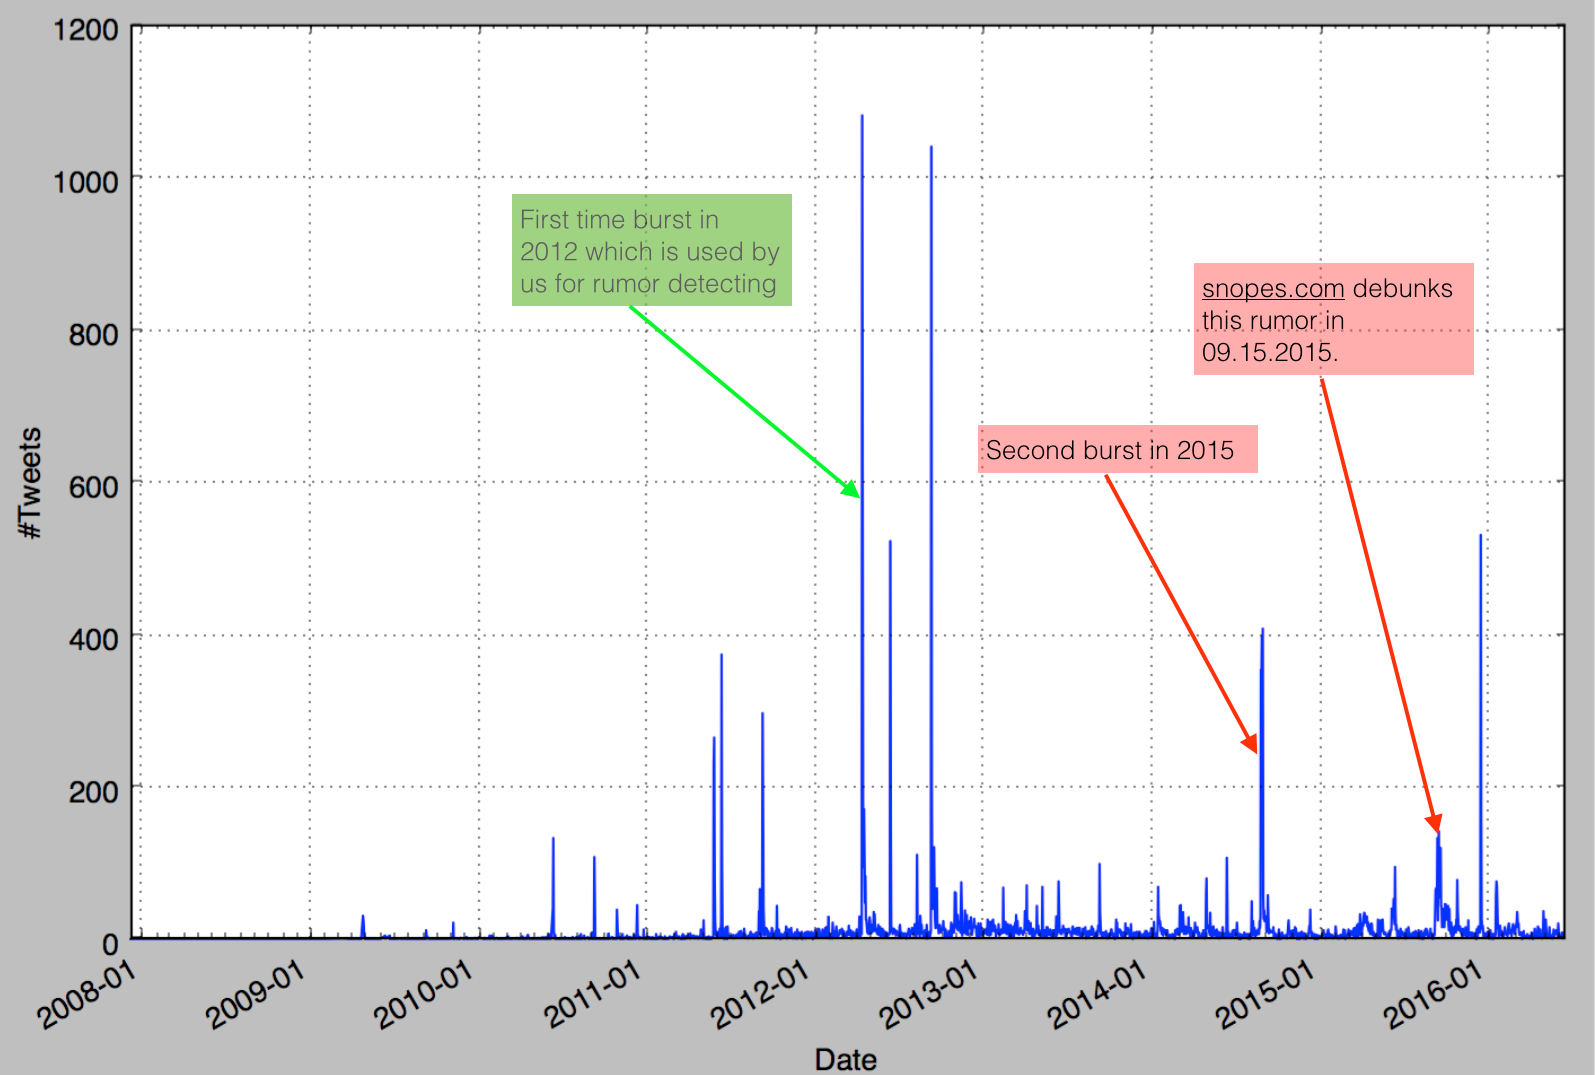
\includegraphics[width=0.8\columnwidth]{images/mutipikehiding.png}
\caption{Tweet Volume of Rumor about Tupac Shakur}
\label{fig:Multipike}
\end{figure}   
   
So we set up a threshold 72 hours. We only consider the first tweet containing snopes in text or URL within 72 hours before or after the beginning time of the event as time stamp of human confirming rumors. We show two examples here. First one in Figure \ref{fig:ealiset_rumo} is a rumor about okra Curing diabetes\footnote{http://www.snopes.com/medical/homecure/okra.asp} which we detected the beginning time is 01.31.2014 04:00. So we scan the first tweet about snopes and we find it in 01.28.2014 21:00 which is 55 hours earlier than the beginning time. Snopes didn't explain their source of this rumor, maybe they detect the story not from Twitter. 
Other example in Figure \ref{fig:lastest_rumo} is that  human detect rumor 71 hour after the event beginning.  
The result is shown in Table \ref{tab:Human_confit_rumor}. On average the editors of "snopes.com" need 25.49 hours to verify the rumors and post it. Our system already achieves 87\% accuracy in 25 hours. 
     \begin{figure}[!h]
\centering
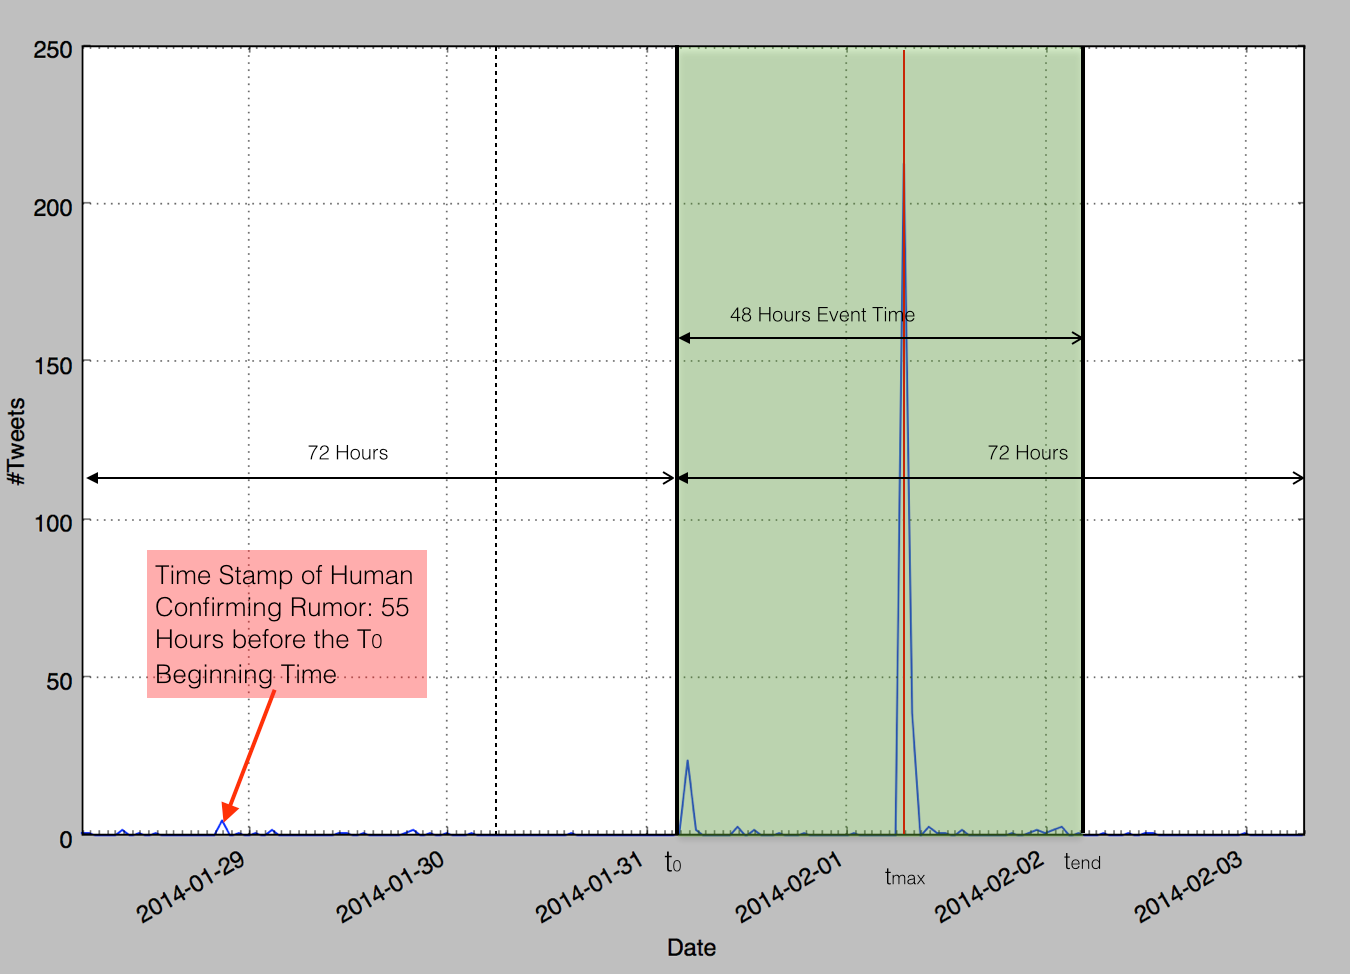
\includegraphics[width=0.8\columnwidth]{images/Timestamphummanearlist.png}
\caption{The Earliest Time Stamp of Human Confirming Rumor}
\label{fig:ealiset_rumo}
\end{figure} 
  \begin{figure}[!h]
\centering
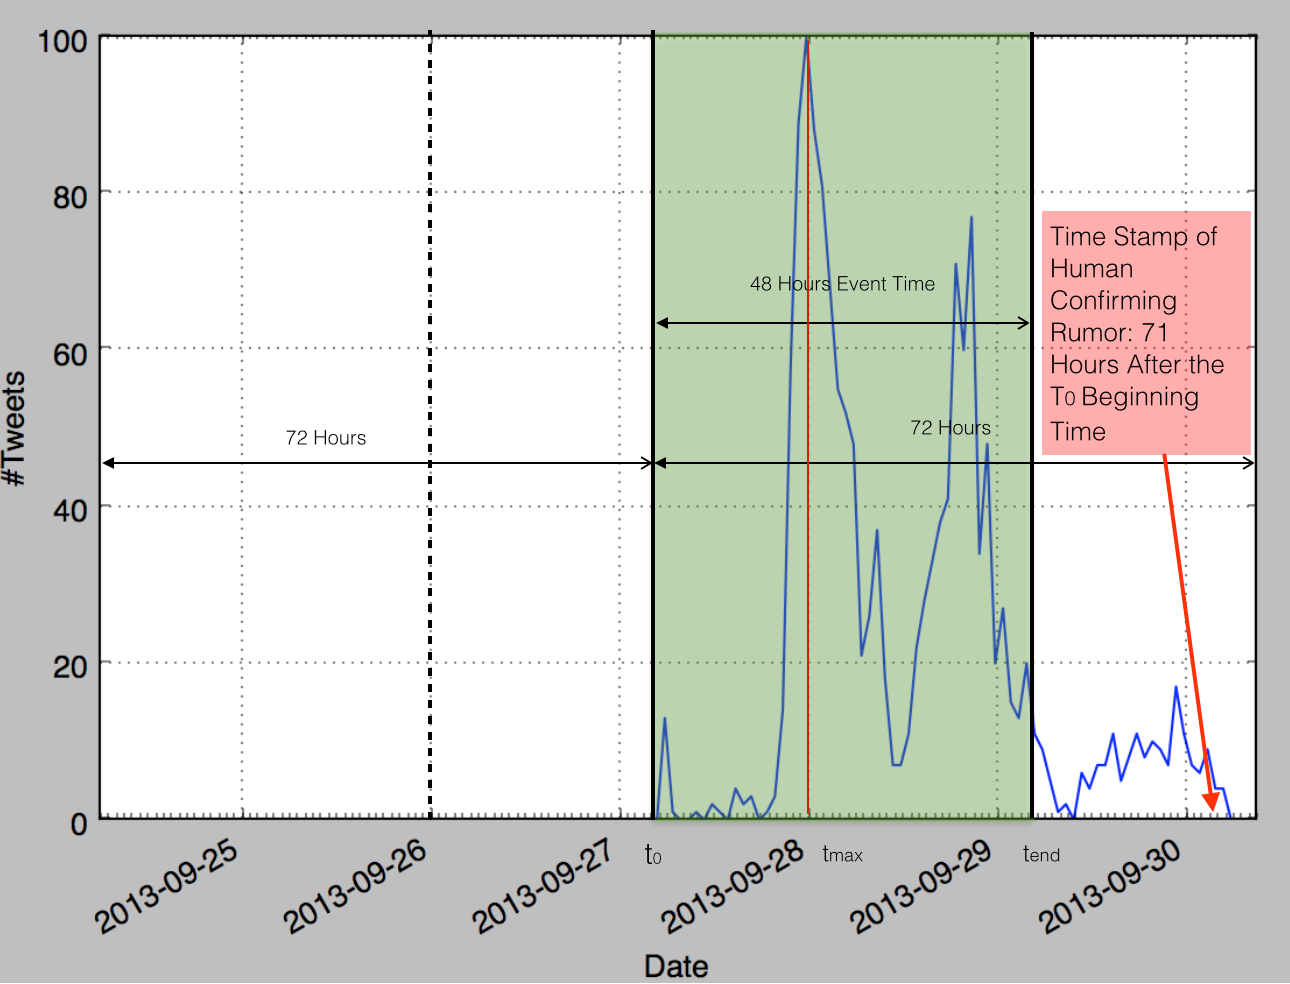
\includegraphics[width=0.8\columnwidth]{images/Timestamphummanlatest.png}
\caption{The Lastest Time Stamp of Human Confirming Rumor}
\label{fig:lastest_rumo}
\end{figure} 
  \begin{table*}[!h]
 \centering
\scalebox{1}{
\begin{tabular}{@{\textbf{ }}cll@{}}
\toprule
\textbf{} & \textbf{Hours} \\ \midrule
Latest Time of Human Detection & 71\\
Earliest Time of Human Detection			& -55\\
Average 		& 25.49\\
\bottomrule

\end{tabular}}
\caption{Time of Human Confirming Rumors }
\label{tab:Human_confit_rumor}
\end{table*}
 
 \clearpage
 \subsection{Discussion } 
 \subsubsection{Why sentiment doesn't work so well in time series model}
 \emph{PolarityScores} is the best feature of single tweet model. But it dose not work well in time series. Generally   the performance of \emph{PolarityScores} drops down over time. 
  In Table \ref{Percentage-of-tweet-type} we reference the result from Thomas Heverin's work \cite{heverin2010microblogging}. He analyzed the tweets which responded to the 2009 Violent Crisis. The number of tweets containing original information and emotion are less and less over time. In the other hand, more and more people start to share their different opinions even technology problems after 24 hours. That may make difference of sentiment features between rumors and news less and less over time and after 24 hours it becomes useless. 
\begin{table}[!h]
\centering
\begin{tabular}{ccccccc}
\hline

\multicolumn{1}{|c|}{\small{Time Period}} & \multicolumn{1}{c|}{\small{Information}} & \multicolumn{1}{c|}{\small{Opinion}} & \multicolumn{1}{c|}{\small{Technology}} & \multicolumn{1}{c|}{\small{Emotion}} & \multicolumn{1}{c|}{\small{Action}} & \multicolumn{1}{c|}{\small{Other}} \\ \hline
\multicolumn{1}{|c|}{\small{0-12hours}}   & \multicolumn{1}{c|}{90.0\%}           & \multicolumn{1}{c|}{6.8\%}        & \multicolumn{1}{c|}{1.1\%}           & \multicolumn{1}{c|}{5.6\%}        & \multicolumn{1}{c|}{1.1\%}       & \multicolumn{1}{c|}{0.0\%}      \\ \hline
\multicolumn{1}{|c|}{\small{12-24 hours}} & \multicolumn{1}{c|}{86.6\%}           & \multicolumn{1}{c|}{13.0\%}       & \multicolumn{1}{c|}{3.1\%}           & \multicolumn{1}{c|}{4.5\%}        & \multicolumn{1}{c|}{1.3\%}       & \multicolumn{1}{c|}{0.7\%}      \\ \hline
\multicolumn{1}{|c|}{\small{24-36 hours}} & \multicolumn{1}{c|}{73.9\%}           & \multicolumn{1}{c|}{18.3\%}       & \multicolumn{1}{c|}{7.0\%}           & \multicolumn{1}{c|}{2.7\%}        & \multicolumn{1}{c|}{0.5\%}       & \multicolumn{1}{c|}{3.7\%}      \\ \hline
\multicolumn{1}{|c|}{\small{26-48 hours}} & \multicolumn{1}{c|}{74.6\%}           & \multicolumn{1}{c|}{21.3\%}       & \multicolumn{1}{c|}{1.0\%}           & \multicolumn{1}{c|}{3.8\%}        & \multicolumn{1}{c|}{0.5\%}       & \multicolumn{1}{c|}{2.8\%}      \\ \hline

\end{tabular}
   \caption{. Percentage of Tweet Type (Non-Exclusive) Per 12 Hour Time Period (Source: \cite{heverin2010microblogging})}
\label{Percentage-of-tweet-type}

\end{table}


  \subsubsection{Performance of External URLs features}
  In this section, We will discuss the performance of external urls features. An interesting phenomenon of  external urls features is their performances is much better 24 hours later after the beginning of the events.
  
  In our experiment, we have 3 features about the external URLs: \emph{ContainNEWS}, \emph{UrlRankIn5000} and \emph{WotScore}. It is clear to see in Table \ref{twitterfeaturerank} that after 24 hours the performances of these features are better than the performances before 24 hours.    
  
  In Alexander's work \cite{mills2009web}, he also shows similar phenomenon that credibility of the information from Twitter is higher than external website in the first 24 hours. That may be the reason why the features of external links performance better after 24 hours.
\ref{fig:informationqulitat}. 
  \begin{figure}[!h]
\centering
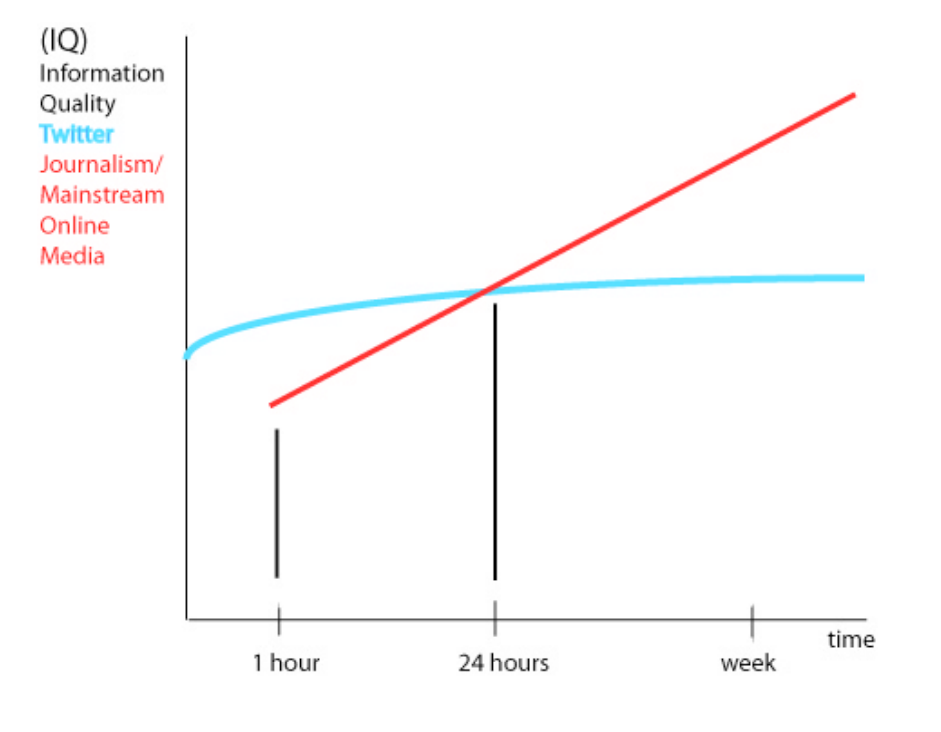
\includegraphics[width=0.7\columnwidth]{images/Informationqulitat.png}
\caption{Information Quality Over Time (source: \cite{mills2009web})}
\label{fig:informationqulitat}
\end{figure}
\newpage
 \subsubsection{Case Study: Munich Shooting } 
 In this section, We will present a case study of Munich shooting. We will show the time line of event and the the performance of our model in the early stage of event. Finally we will discuss some example of the misclassification of our single tweet's credibility model.
 
 The time of the event:
 \begin{itemize}
 	
 
\item  At 17:52 CEST a shooter opened fire in the vicinity of the Olympia shopping mall in Munich. 10 people, including the shooter, were killed and 36 others were injured\footnote{https://en.wikipedia.org/wiki/2016\_Munich\_shooting}. 

\item  At 18:22 CEST first tweet was posted. It might contain some delay here, because our query is constructed in English and maybe the very first tweets are in German. The tweet is \emph{"Sadly, i think there's something terrible happening in \#Munich \#Munchen. Another Active Shooter in a mall. \#SMH"}. 
\item At 18:25 CEST the second tweet was posted: \emph{"Terrorist attack in Munich????"}.   

\item  At 18:27 CEST the traditional media (BBC) posted their first tweet. \emph{"'Shots fired' in Munich shopping centre - http://www.bbc.co.uk/news/world-europe-36870800a02026 @TraceyRemix gun crime in Germany just doubled"}.

\item At 18:31 CEST, the first misclassified tweet is posted. It was a tweet with shock sentiment and swear words: \emph{"there's now a shooter in a Munich shopping centre.. What the fuck is going on in the world. Gone mad"}.
\end{itemize}

We show the \emph{CreditScore} of Munich Shooting event in Figure \ref{fig:munichattackCS}. It is clear to see that the event Munich Shooting has higher \emph{CreditScore} than the average of news events. But we labeled all the tweets about Munich shooting as news related, but because this event contains a large tweets' volume and there must be some rumors spreading with it. It may cause the single tweet credibility model unreliable. But we use the average CreditScore of the event as features, it can limit the influence of the defects of ground-truth.
  \begin{figure}[!h]
\centering
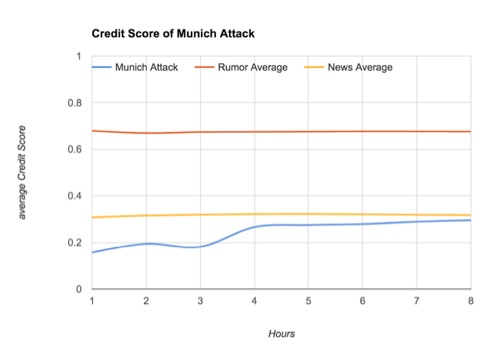
\includegraphics[width=0.7\columnwidth]{images/munichCD.png}
\caption{CreditScore of Munich Shooting Comparing With Average CreditScore of 130 Rumors and 130 News}
\label{fig:munichattackCS}
\end{figure}

There are several kinds of misclassification shown in Table 
\ref{tab:Munshot}: 
unrelated to the events, strong emotional and rumor related:
\begin{itemize}
	\item We searched the tweet in English, so most users are in America not in Germany who can talk about some extend topics like gun law. These comments are labeled as rumors by our system. 
\item And some tweets contain strong personal emotion even swear words. These tweets have higher probability being labeled as rumor. 
\item The third type is rumor. Some rumors were spreading with the news events. For example some tweets claimed Sam Hyde was the shooter and posted a photo with an armed man on it. Or some claimed the shooter was a member of ISIS. They are also detected by our system. But generally the average CreditScore is more like a news event.
\end{itemize}

 
\begin{table*}[!h]
 \centering
\scalebox{1}{
\begin{tabular}{@{\textbf{ }}cp{350pt}@{}}
\toprule
\textbf{Catalogue} & \textbf{Examples of Tweets} \\ \midrule
\multirow{2}{*}{Event Unreleted} & Looks like the EU's gun ban has continued to do its job. What a success. \#Munich https://twitter.com/RT\_com/status/756525863093538817\\\cline{2-2} 
 			& The strict gun laws in Munich kept guns out of innocent hands, didn't stop the terrorists, in fact made their job easier. @realDonaldTrump\\\cline{2-2}
 	&	@KummersTim @ShepNewsTeam Shep Smith is colluding with Hillary's camp also what he tried during Munich attack was disgusting \#TrumpPence16	\\
 			\midrule
\multirow{2}{*}{Strong Emotional}  & Munich Another day another attack. when is this shit gonna end. It is becoming the norm now. Saddening .\\ \cline{2-2} 
 			& there's now a shooter in a Munich shopping centre.. What the fuck is going on in the world. Gone mad\\\midrule
Rumors			& ISIS On Munich Terror Attack: Everything Hurting Infidels Makes Us Happy http://www.weaselzippers.us/285113-isis-on-munich-terror-attack-everything-hurting-infidels-makes-us-happy/ via @WeaselZippers\\ \cline{2-2}
			& Obama released photo of shooter \#Munich pic.twitter.com/GzJkyNpYDP\\\cline{2-2}
			& Nice attack 7 days ago, Wurzburg axe attack Monday, Alps knife attack on Wednesday \& Munich shootings ongoing. All are Jihad, get used to it\\\cline{2-2}
			& New info: Munich shooter has been consuming high amounts of a chemical substance called \"H2O\"! \#banH2O \#banChemistry \\\cline{2-2}
			& @M7madSmiry @TheBpDShow hearing reports that the shooter is a white supremacist... Has that been confirmed? \#Munich\\\cline{2-2}
			& Witness In Munich Shooting Says: The Shooter Cried Out Allahu Akbar As He Slaughtered Children http://shoebat.com/2016/07/22/witness-in-munich-shooting-says-the-shooter-cried-out-allahu-akbar-as-he-slaughtered-children/  via @walidshoebat\\\midrule
others &	@ThatTimWalker seems you were wrong re the Munich attack.\\
		
 			\bottomrule

\end{tabular}}
\caption{Example of Misclassification by Single Tweet Model on Munich Shotting}
\label{tab:Munshot}
\end{table*}
  \begin{figure}[!h]
\centering
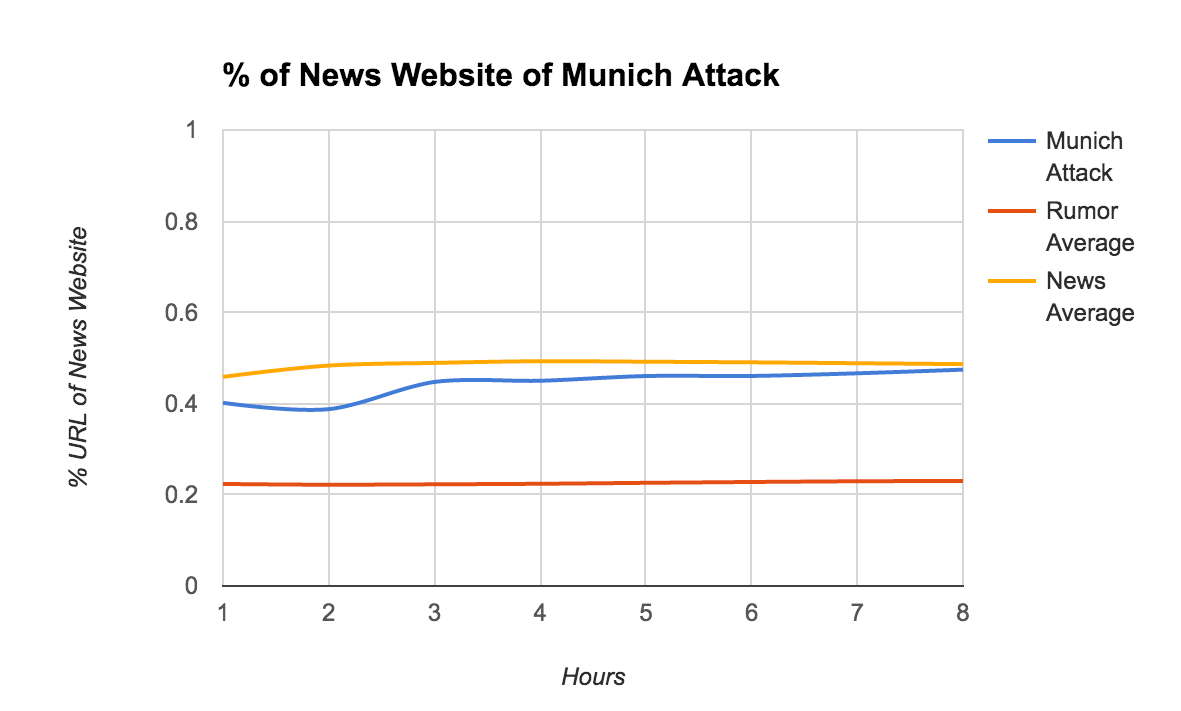
\includegraphics[width=0.8\columnwidth]{images/munichNews.png}
\caption{\% of Tweet Containing News Websites of Munich Shooting Comparing With Average ContainNews of 130 Rumors and 130 News}
\label{fig:munichattackNews}
\end{figure}

The second best feature is ContainNews which is the percent number of the URLs containing News Website. We show the ContainNews of Munich attack in Figure \ref{fig:munichattackNews}. 
 We can see the curve of ContainNews of Munich shooting event is closer to the curve of ContainNews average News events. 
 
